\documentclass[11pt]{article}
\usepackage{deauthor}
\usepackage[T1]{fontenc}
\usepackage[latin9]{inputenc}
\usepackage{enumitem}
\usepackage{sidecap}
\usepackage{framed}
\usepackage{cprotect}
\usepackage{enumitem}
\usepackage{listings}
\usepackage{amstext}
\usepackage{amstext}
\usepackage{pdfpages}
\usepackage{alltt}
\usepackage{epstopdf}
\usepackage{xspace,colortbl}
\usepackage[USenglish]{babel}
\usepackage{multirow}
\usepackage{url}
\usepackage{subfigure}
\usepackage{graphicx}%%
\usepackage{amssymb}
\usepackage{fmtcount}
\usepackage{amsfonts}
\usepackage{xspace}
\usepackage{amsmath}
\usepackage{multirow}
\usepackage[mathscr]{eucal}
%\usepackage{psfrag}
\usepackage{colortbl}

\usepackage{bm}
\usepackage{times}
\usepackage[nospace]{cite}
\usepackage{csquotes}
\usepackage{enumitem}
\usepackage{geometry}
%\geometry{verbose,tmargin=2.54cm,bmargin=2.54cm,lmargin=2.54cm,rmargin=2.54cm}
\usepackage{babel}
\begin{document}

%\newtheorem{theorem}{Theorem}
%\newtheorem{example}{Example}
%\newtheorem{definition}{Definition}
%\newtheorem{problem}{Problem}
%\newtheorem{property}{Property}
%\newtheorem{proposition}{Proposition}
%\newtheorem{lemma}{Lemma}
%\newtheorem{corollary}{Corollary}

\newcommand{\cond}{\textrm{pred}\xspace}
\newcommand{\dataset}{data set\xspace}
\newcommand{\datasets}{data sets\xspace}
\newcommand{\spview}{\textsf{SPView}\xspace}
\newcommand{\fjview}{\textsf{FJView}\xspace}
\newcommand{\aggview}{\textsf{AggView}\xspace}
\newcommand{\hashfunc}[1]{\textsf{hash}(#1)\xspace}
\newcommand{\hashop}{\textsf{hash}\xspace}
\newcommand{\nsc}{\textsf{NormalizedSC}\xspace}
\newcommand{\rsc}{\textsf{RawSC}\xspace}

\newcommand{\avgfunc}{\ensuremath{\texttt{avg} }\xspace}
\newcommand{\maxfunc}{\ensuremath{\texttt{max} }\xspace}
\newcommand{\minfunc}{\ensuremath{\texttt{min} }\xspace}
\newcommand{\histfunc}{\ensuremath{\texttt{histogram\_numeric} }\xspace}
\newcommand{\countfunc}{\ensuremath{\texttt{count}}\xspace}
\newcommand{\sumfunc}{\ensuremath{\texttt{sum} }\xspace}
\newcommand{\varfunc}{\ensuremath{\texttt{var} }\xspace}
\newcommand{\stdfunc}{\ensuremath{\texttt{std} }\xspace}
\newcommand{\covfunc}{\ensuremath{\texttt{cov} }\xspace}
\newcommand{\corrfunc}{\ensuremath{\texttt{corr} }\xspace}
\newcommand{\medfunc}{\ensuremath{\texttt{median} }\xspace}
\newcommand{\percfunc}{\ensuremath{\texttt{percentile} }\xspace}
\newcommand{\havingfunc}{\ensuremath{\texttt{HAVING} }\xspace}
\newcommand{\selectfunc}{\ensuremath{\texttt{select} }\xspace}
\newcommand{\ratio}{\ensuremath{\rho }\xspace}
\newcommand{\mean}{\ensuremath{\texttt{mean} }\xspace}
\newcommand{\pred}{\ensuremath{\texttt{pred} }\xspace}

\newcommand{\insertion}{\ensuremath{\texttt{INSERT} }\xspace}
\newcommand{\update}{\ensuremath{\texttt{UPDATE} }\xspace}
\newcommand{\delete}{\ensuremath{\texttt{DELETE} }\xspace}
\newcommand{\svc}{View Cleaning\xspace}

\newcommand{\saqpfunc}{\ensuremath{\phi }\xspace}
\newcommand{\saqpplusfunc}{\ensuremath{\phi_{\clean} }\xspace}
\newcommand{\clean}{\ensuremath{\texttt{clean} }\xspace}
\newcommand{\sampleclean}{SampleClean\xspace}

\newcommand{\Correct}[1]{\texttt{Correct}\ensuremath(#1)\xspace}
\newcommand{\Remove}[2]{\texttt{Remove}\ensuremath(#1, #2)\xspace}
\newcommand{\Predicate}[1]{\texttt{Predicate}($#1$)\xspace}
\newcommand{\Predicaten}[1]{\texttt{Predicate}(#1)\xspace}
\newcommand{\Predicatec}[1]{\texttt{Predicate}(\texttt{Correct}($#1$))\xspace}
\newcommand{\Dedup}[2]{\texttt{Numdup}\ensuremath(#1)\xspace}

\newcommand{\jn}[1]{\textcolor{red}{\{\{JN: #1\}\}}\xspace}

\def\ojoin{\setbox0=\hbox{$\bowtie$}% 
  \rule[-.02ex]{.25em}{.4pt}\llap{\rule[\ht0]{.25em}{.4pt}}}
\def\leftouterjoin{\mathbin{\ojoin\mkern-5.8mu\bowtie}}
\def\rightouterjoin{\mathbin{\bowtie\mkern-5.8mu\ojoin}}
\def\fullouterjoin{\mathbin{\ojoin\mkern-5.8mu\bowtie\mkern-5.8mu\ojoin}}

\setlength{\belowdisplayskip}{1pt} \setlength{\belowdisplayshortskip}{1pt}
\setlength{\abovedisplayskip}{1pt} \setlength{\abovedisplayshortskip}{1pt}

\author{ Sanjay Krishnan$^1$, Jiannan Wang$^1$, Michael J. Franklin$^1$, Ken Goldberg$^1$,\\
Tim Kraska$^2$, Tova Milo$^3$, Eugene Wu$^4$\\ \\
$^1$UC Berkeley,~~$^2$Brown University,~~$^3$Tel Aviv University,~~$^4$Columnia University \\
%\{jnwang, sanjaykrishnan, franklin, goldberg\}@berkeley.edu\\
%milo@cs.tau.ac.il,tim\_kraska@brown.edu,ewu@columbia.edu
}

\title{SampleClean: Fast and Reliable Analytics on Dirty Data}
\maketitle
\begin{abstract}
An increasingly important challenge in data analytics is dirty data in the form of missing, duplicate, incorrect, or inconsistent values.  
In the SampleClean project, we have developed a new suite of algorithms to estimate the results of different types of analytic queries after applying data cleaning only to a sample.
First, This article describes methods for computing statistically bounded estimates of SUM, COUNT, and AVG queries from samples of data corrupted with duplications and incorrect values.
Some types of data error, such as duplication, can affect sampling probabilities so results have to be re-weighted to compensate for biases.
Then it presents an application of these query processing and data cleaning methods to materialized views maintenance.
The view cleaning algorithm applies hashing to efficiently maintain a uniform sample of rows in a materialized view, and then dirty data query processing techniques to correct stale query results.
Finally, the article describes a gradient-descent algorithm that extends this idea to the increasingly common Machine Learning-based analytics.
\end{abstract}

\section{Introduction}
Data are susceptible to various forms of corruption such as missing,
incorrect, or inconsistent representations \cite{Gartner}.
Real-world data is commonly integrated from multiple sources, and the integration process may lead to a variety of data errors~\cite{DBLP:journals/pvldb/DongS13}. 
Data analysts report that data cleaning remains one of the most time
consuming steps in the analysis process \cite{nytimes}.
Identifying and fixing data error often requires manually inspecting data, which can quickly become costly and time-consuming. 
While crowdsourcing is an increasingly viable option for some types of errors ~\cite{DBLP:conf/sigmod/JefferyFH08,DBLP:journals/pvldb/FanLMTY10,DBLP:journals/pvldb/YakoutENOI11, gokhale2014corleone, park2014crowdfill, sampleclean,chu2015katara}, it comes at the significant cost of additional latency and the overhead of managing human workers. 

Ignoring the effects of dirty data is potentially dangerous.
Since \emph{a priori}, the magnitude of data error is unknown, any amount of error can be biasing.
Analysts have to choose between facing the cost of data cleaning
or coping with consequences of unknown inaccuracy.
In this article, we describe a middle ground that we call SampleClean \cite{wang1999sample, krishnan2015svc}; where an analyst can clean a sample of data, and use this sample to improve an erroneous query result.
The intriguing part of SampleClean is that while the query result is computed using a sample,                                   
results can often be more accurate than those computed over the full data due to the data cleaning.
This approximation error is boundable unlike the unknown data error, and the tightness of the bound is parametrized by a flexible cleaning cost (i.e., the sampling ratio).

The case for SampleClean is analogous to the case for Approximate Query Processing \cite{DBLP:conf/icde/OlkenR92, olken1993random, garofalakis2001approximate, AgarwalMPMMS13} (AQP).
For decision problems, exploratory analysis problems, and visualization, it often suffices to return an approximate query result bounded in confidence intervals; thus saving significant processing costs.
In many common aggregates, the samples-to-accuracy trade off tends to vary as $O(\frac{1}{\sqrt{n}})$, and therefore every additional $\epsilon$ factor of accuracy costs quadratically more. 
In applications where approximation can be tolerated, sampling avoids the expensive ``last mile" of processing and timely answers facilitate improved user experiences and faster analysis.

In traditional AQP, approximation necessarily sacrifices accuracy for reduced latency. 
However, the goal of SampleClean differs from AQP, as SampleClean trades off data transformation cost for gradual improvements in query accuracy through data cleaning.
While SampleClean introduces approximation error, the data cleaning mitigates errors in query results.
There is a break-even point where a sufficient amount of data is cleaned to facilitate an accurate approximation of queries on the cleaned data, and in this sense, sampling actually improves the accuracy of the query result.

SampleClean \cite{wang1999sample} and all of its extensions \cite{krishnan2015svc}, work in the \emph{budgeted data cleaning} setting. 
An analyst is allowed to apply an expensive data transformation $C(\cdot)$ to only $k\ll N$ rows in a relation.
One solution could be to draw $k$ records uniformly at random and apply data cleaning, e.g., a direct extension of AQP to the cleaned sample.
However, data cleaning presents a number of methodological problems that make this hard.
First, $C(\cdot)$ may change the sampling statistics, for example, duplicated records are more likely to be sampled.
Next, query processing on partially clean data, i.e., a mix of dirty and clean data, can lead to unreliable results due to the well known Simpsons Paradox.
Finally, high-dimensional analytics such as Machine Learning may be very sensitive to sample size, perhaps even more so than to dirty data, and techniques for avoiding sample size dependence are required.

One of the key insights is that there are two contrasting query processing techniques to address every budgeted data cleaning problem.
A direct extension of AQP can estimate the true query result based on the cleaned sample (possibly with some reweighting to account for changes in sampling statistics). 
A sample of cleaned data can also be used to correct the error in a query result over the dirty data.
There is an interesting theoretical tradeoff between these approaches, where the first approach is \emph{robust} as its accuracy is independent of the magnitude of data error, and the second approach is \emph{sample-efficient} as its accuracy is less dependent on sample size.

By establishing the link between AQP and data cleaning, this idea has opened up a number of new research opportunities. 
We applied the same principles to other domains with expensive data transformations such as Materialized View Maintenance and Machine Learning.
In this article, we highlight four projects:

\vspace{0.5em}
\noindent \textbf{\sampleclean \cite{wang1999sample}: } \sampleclean estimates aggregate (\sumfunc, \countfunc, \avgfunc) queries using samples of clean data. \sampleclean reweights the data to compensate for changes in sampling statistics such that the estimates are unbiased and bounded in confidence intervals.

\vspace{0.5em}
\noindent \textbf{View Cleaning \cite{krishnan2015svc}: } View Cleaning generalizes the notion of data cleaning to include expensive maintenance of out-of-date data. Staleness in materialized views (MVs) manifests itself as data error, i.e., a stale view has missing, superfluous, and incorrect rows.
Like data cleaning, eager MV maintenance is expensive, and View Cleaning models querying an MV as a budgeted data cleaning problem.
Aggregate queries are approximated from a stale MV using a small sample of up-to-date data, resulting in bounded estimates.

\vspace{0.5em}
\noindent \textbf{ActiveClean: } ActiveClean extends \sampleclean to a class of analytics problems called Convex Data Analytics (subsuming the aggregates studied in \sampleclean and including Machine Learning such as Support Vector Machines and Linear Regression). ActiveClean exploits the convex structure of the problem (i.e. gradients and feature space) to prioritize cleaning data that is likely to affect the model. ActiveClean directly integrates cleaning into the model training loop and as a result gives a bounded approximation for any cleaning budget.

\vspace{0.5em}
\noindent \textbf{Wisteria \cite{haas2015wisteria}: } Wisteria is a system that implements the ideas described in the SampleClean work in a distributed analytics platform. This involved designing an algebra for data cleaning transformations and optimizations for their execution to reduce the latency of data cleaning operators.

\vspace{0.5em}

This article is organized as follows. Section 2 introduces the project and its main ideas. Section 3 overviews the basic architecture of each one of the projects. Section 4/5/6 describes \sampleclean, View Cleaning, and ActiveClean respectively. Section 7 reviews the related work in this field. In Section 8, we highlight some of the open problems and future directions of the SampleClean project. Finally, we conclude in Section 9.
\section{Background and Main Ideas}

This section describes the key idea of SampleClean, namely, that data cleaning can be integrated with approximate query processing leading to bounded approximations of clean query results for a fraction of the cleaning cost.

\subsection{Data Cleaning is Often Expensive}
A number of surveys report that data cleaning is one of the most time consuming steps \cite{kandel2012enterprise, nytimes}.
Data cleaning frameworks have been recently proposed to address the problem of corrupted data at scale\cite{khayyat2015bigdansing, chu2015katara, sampleclean}.
As errors can be domain- or dataset-specific, data cleaning is an inherently human-driven process and can require a significant amount of developer effort in writing software or rules to fix the corruption.
Automated fixes may not be reliable and can require human confirmation \cite{DBLP:journals/pvldb/YakoutENOI11}.
One way to scale up human computation is crowdsourcing which has shown recent success in entity resolution and value filling \cite{gokhale2014corleone, park2014crowdfill, sampleclean,chu2015katara}.
However, crowdsourcing comes with the costs of significant additional latency (orders of magnitude slower than data processing) and the overhead of managing human workers.

\subsection{Traditional Approximate Query Processing}
The basic idea of AQP is to approximate the result of a query $Q$ on a large relation $R$, instead of processing the entire relation.
A number of approximation schemes have been proposed including using Sampling, Wavelets, Sketching, and Hashing (see Cormode et al. for a survey \cite{DBLP:journals/ftdb/CormodeGHJ12}).
This article focuses on Sampling-based approximations.
Sampling-based approximate query processing (SAQP) is a powerful technique that allows for fast approximate results on large datasets. 
It has been well studied in the database community since the 1990s~\cite{DBLP:conf/sigmod/HellersteinHW97,DBLP:conf/sigmod/AcharyaGPR99,DBLP:conf/icde/OlkenR92, OlkenR86}, and methods such as BlinkDB~\cite{DBLP:conf/eurosys/AgarwalMPMMS13} have drawn renewed attention in recent big data research. 
An important aspect of SAQP is confidence intervals, as many types of aggregates can be bounded with techniques such as concentration inequalities (e.g., Hoeffding bounds), large-deviation inequalities (e.g., Central Limit Theorem), or empirically (e.g., Bootstrap). 

Suppose, there is a relation $R$ and a uniform sample $S$.
SAQP applies a query $Q$ to $S$ (possibly with some scaling $c$) to return an estimate: 
\[
Q(R) \approx est = c \cdot Q(S)
\]

Traditionally, AQP sacrifices accuracy due to sampling for improved query latency.
However, bounds on $est$ assume that the only source of error is uncertainty introduced by sampling, however, the data itself may contain errors which could also affect query results.
When the data itself is erroneous, a query result on the full data--let alone a sample, will be incorrect.
The main argument for SampleClean is that when data errors significantly affect query results,
sampling can be combined with data cleaning to actually improve accuracy.
This leads to a counter-intuitive result where it is possible that a query on a cleaned sample of data is more accurate than a query on the entire dirty data.

\iffalse
\subsection{Exploiting Application Structure}

\jn{It's a little too early to present the content of this section before showing the big idea. I would suggest to put it either to the end of Sec 2 or the end of Sec 3. }

SampleClean applies sample to clean $k\ll N$ rows in a database to address the time-scale mismatch between the analytics application (e.g., SQL query, Machine Learning, Materialized View) and data cleaning.
An important aspect of this project is how the structure and semantics of that application can be used to prioritize and budget data cleaning.
A database only needs to be sufficiently clean for the requirements of the subsequent analytics--and the key insight from AQP being that aggregates are tolerant to approximation.

In the initial SampleClean work, we restricted the allowed aggregate queries to \sumfunc, \countfunc, and \avgfunc with predicates and group by clauses.
In the two subsequent projects, View Cleaning and ActiveClean, we expanded the scope and the semantics of the application. 
The View Cleaning problem explores data cleaning and general aggregates on derived relations with known view definitions.
We can exploit view definition to query just as much of the base data as needed to accurately answer the aggregate query for a fixed budget.
In fact, we showed that any aggregate (beyond \sumfunc, \countfunc, and \avgfunc) that could be estimated with SAQP\cite{agarwalknowing}, could be answered estimated with the View Cleaning framework.
ActiveClean generalizes the initial work on \sumfunc, \countfunc, and \avgfunc to higher-dimensional aggregates.
We defined a class of analytics called Convex Data Analytics, and show how the convex structure of the analytics can be used to guide and prioritize data cleaning.
\fi

\subsection{Approximate Query Processing on Dirty Data}


\subsubsection{Two Sources of Errors: Sampling Error and Data Error}
Now consider the case when the data is dirty.
If $R$ is dirty, then there is a true relation $R_{clean}$.
\[
Q(R_{clean}) \ne Q(R) \approx est = c \cdot Q(S)
\]
The error in $est$ has two components: error due to sampling $\epsilon_s$ and error due to the difference with the cleaned relation $\epsilon_c = Q(R_{clean}) - Q(R)$:
\[
\mid Q(R_{clean}) - est \mid \le \epsilon_s + \epsilon_c
\]

While they are both forms of query result error, $\epsilon_s$ and $\epsilon_c$ are very different quantities.
$\epsilon_s$ is a random variable due to the sampling, and different samples would result in different realizations of $\epsilon_s$.
As a random variable introduced by sampling, $\epsilon_s$ can be bounded by a variety of techniques as a function of the sample size.
On the other hand, $\epsilon_c$ is deterministic, and by definition is an unknown quantity until all the data is cleaned.
Thus, the bounds returned by a typical AQP framework on dirty data would neglect $\epsilon_c$.

It is possible that $R_{clean} \ne R$ but $\epsilon_c=0$.
Consider a \sumfunc query on the relation $R(a)$, where $a$ is a numerical attribute.
If half of the rows in $R$ is corrupted with $+1$ and the other half are corrupted with $-1$, then $Q(R_{clean}) = Q(R)$.
The interesting problem is when there are \emph{systematic errors}\cite{taylor1982introduction} i.e., $\epsilon_c > 0$. 
In other words, the corruption that is correlated with the data, e.g., where every record is corrupted with a $+1$.

\subsubsection{Key Idea I: Direct Estimate vs. Correction}
The key quantity of interest in this work is $\epsilon_c$, and to be able to bound
a query result on dirty data, requires that $\epsilon_c$ is 0 or bound $\epsilon_c$.
There are two ways in which this can be done: direct estimates and corrections.

\vspace{0.5em}
\noindent\textbf{Direct Estimate (Figure \ref{fig:est}A): } This technique is a direct extension of SAQP to handle data cleaning. A set of $k$ rows is sampled uniformly at random from the dirty relation $R$ resulting in a sample $S$. Data cleaning is applied to the sample $S$ resulting in $S_{clean}$.
Data cleaning and sampling may change the statistical and scaling properties of the query $Q$, so $Q$ may have to be re-written to a query $\widehat{Q}$. $\widehat{Q}$ is applied to the sample $S_{clean}$ and the result is returned. 
There are a couple of important points to note about this techniques.
First, as in SAQP, the direct estimate only processes a sample of data.
Next, since it processes a cleaned sample of data, at no point is there a dependence on the dirty data.
As we will show later in the article, the direct estimate returns a result whose accuracy is independent of the magnitude or rate of data error. 
From a theoretical perspective, for some types of data cleaning, this technique ensures that $\epsilon_c = 0$ within the sample.

\vspace{0.5em}
\noindent\textbf{Correction (Figure \ref{fig:est}B): } The direct estimate suffers a subtle drawback. Suppose, there are relatively few errors in the data. The errors introduced by sampling may dominate any error reductions due to data cleaning. Instead of the direct estimate which ensures $\epsilon_c = 0$, we can try to estimate $\epsilon_c$. A set of $k$ rows is sampled uniformly at random from the dirty relation $R$ resulting in a sample $S$. Data cleaning is applied to the sample $S$ resulting in $S_{clean}$. 
The difference in applying $\widehat{Q}$ to S and $\widehat{Q}$ to $S_{clean}$ gives an estimate of $\epsilon_c$. 
The interpretation of this estimate is a correction to the query result on the full dirty data.
In contrast to the direct estimate, this technique requires processing the entire dirty data (but only cleaning a sample).
However, as we will later show, if errors are rare this technique gives significantly improved accuracy over the direct estimates.

\begin{SCfigure}\centering
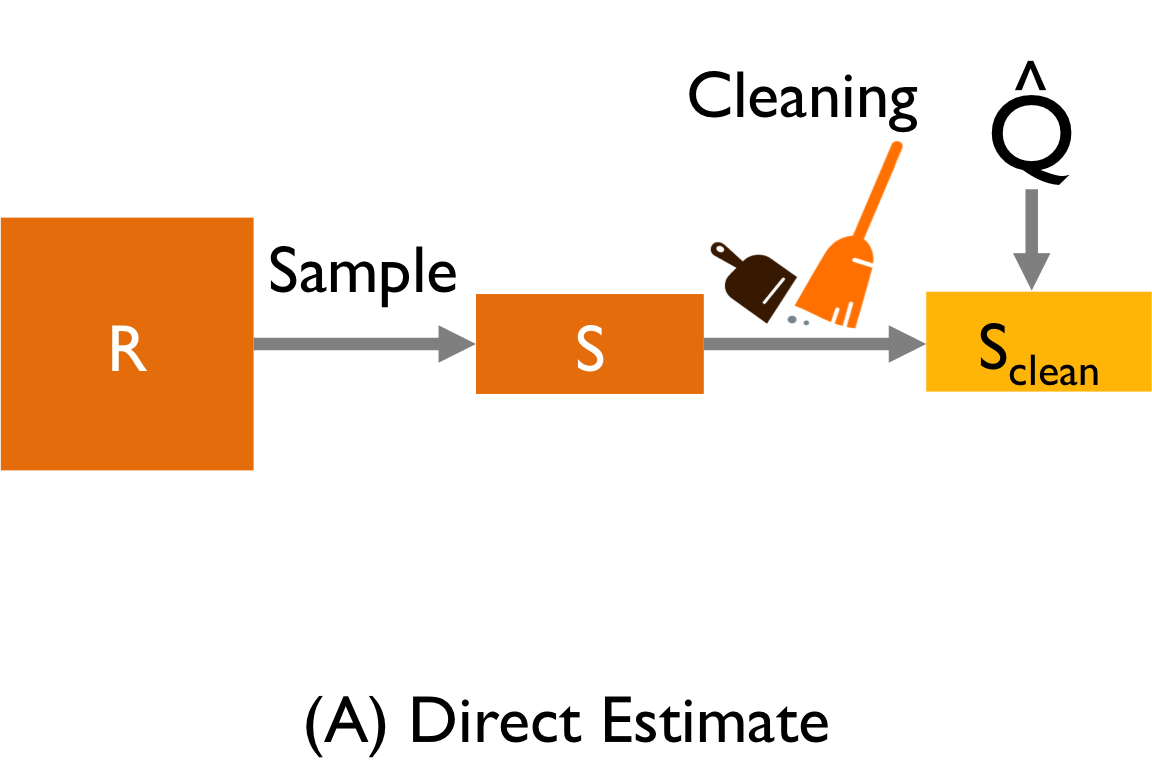
\includegraphics[width=.3\columnwidth]{figs/est1b.png}
\hspace{2em}
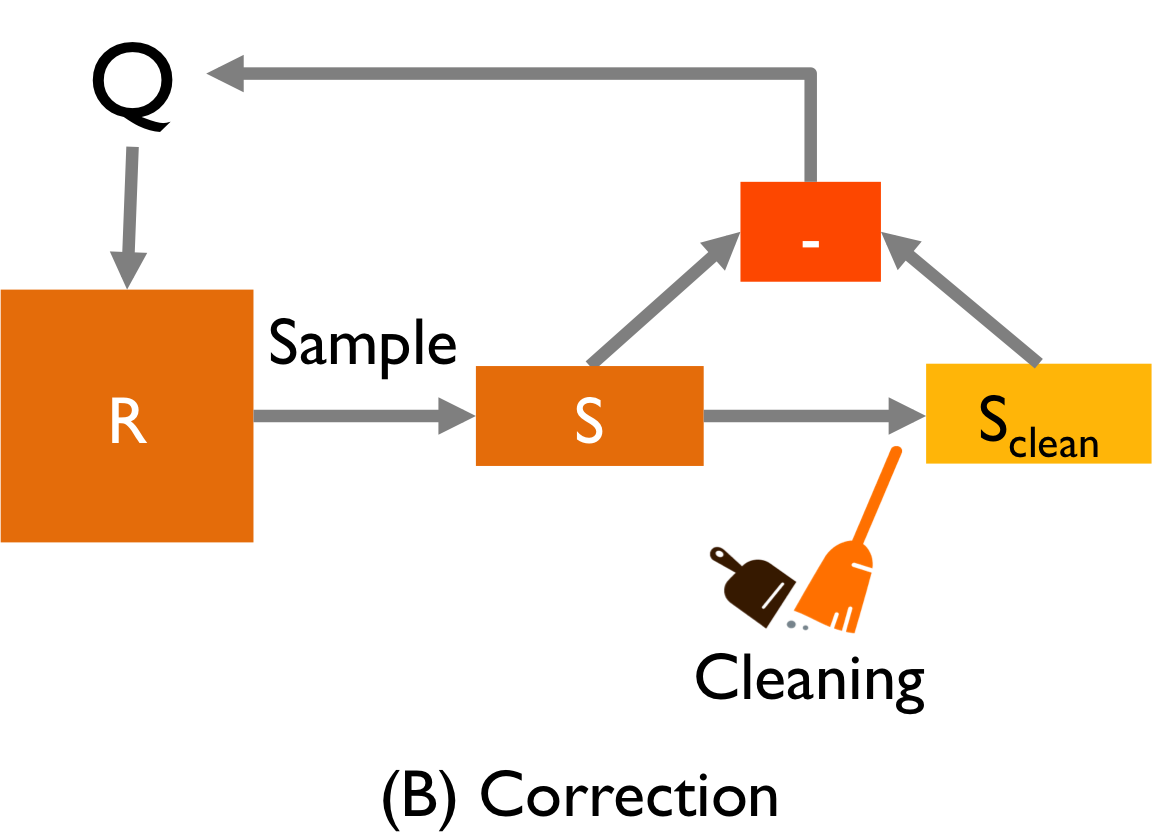
\includegraphics[width=.3\columnwidth]{figs/est1c.png}
\caption{Estimating query results with data cleaning on random samples. There are two ways to estimate a query result: (a) direct estimation applies the query to a sample (possibly with some scaling), and (b) correction corrects a query result on the entire dirty data.\label{fig:est}}
\end{SCfigure}

\subsubsection{Key Idea II: Sampling to Improve Accuracy}
A small sample of clean data can improve improve query accuracy accuracy.
Figure \ref{fig:est2} plots error as a function of the cleaned sample size on a corrupted TPCH dataset for a direct estimate, correction, and AllDirty (query on the full dirty data).
In both cases, there is a break-even point (in terms of number of cleaned samples) when the data cleaning has mitigated more data error than the approximation error introduced by sampling.
After this point, SampleClean improves query accuracy in comparison to AllDirty.
When errors are relatively rare (5\% corruption rate), the correction is more accurate. 
When errors are more significant (50\% corruption rate), the direct estimate is more accurate.
Note that the direct estimate returns results of the same accuracy regardless of the corruption rate. 

\begin{SCfigure}
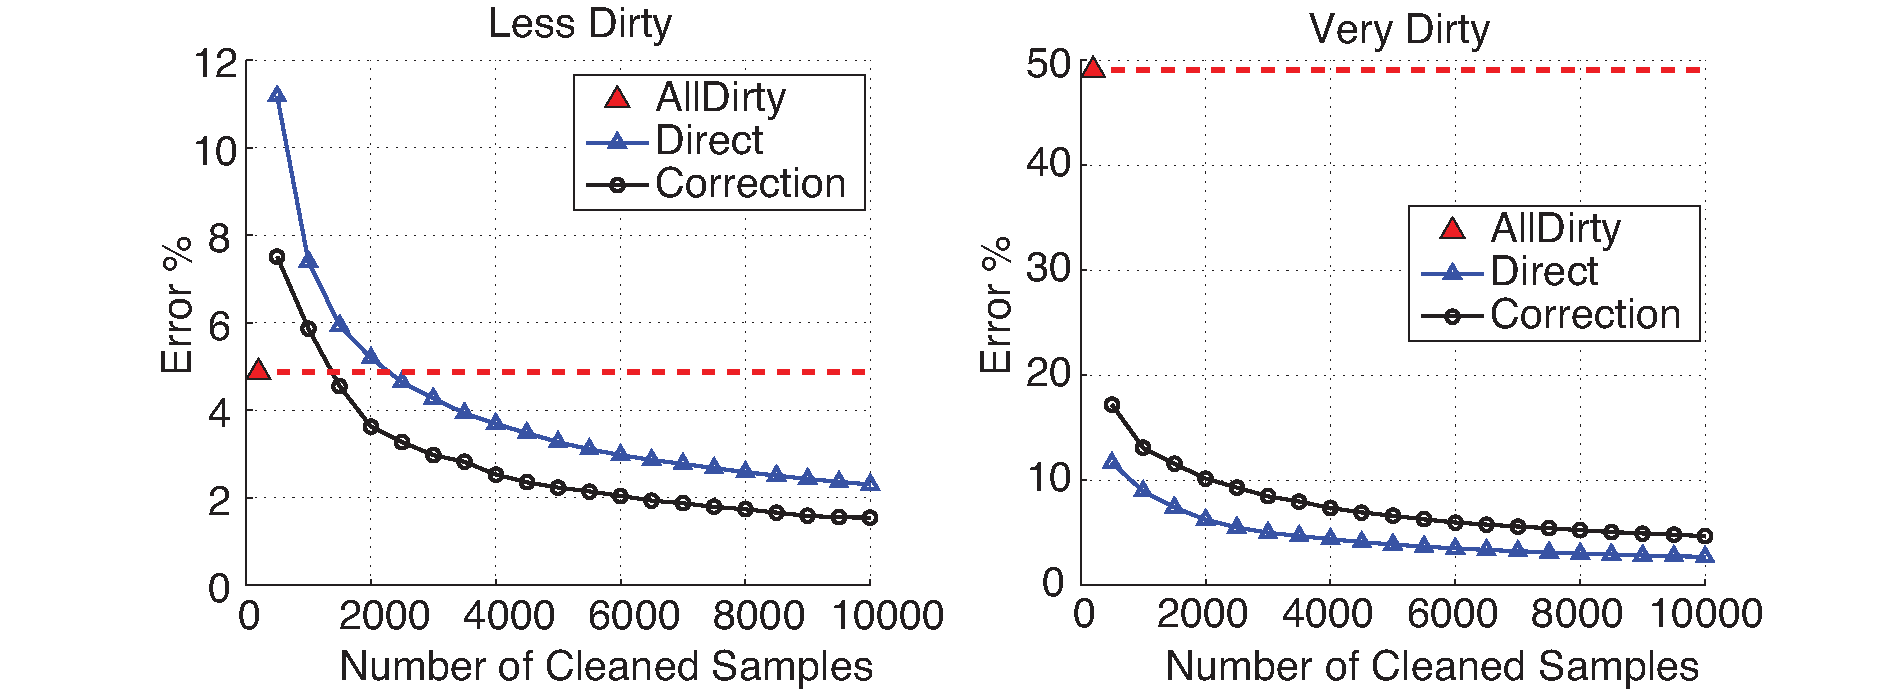
\includegraphics[width=.6\columnwidth]{figs/allerror-samplesize.pdf}
\caption{Comparison of the convergence of the methods on two TPC-H datasets of 6M tuples with simulated errors 50\% error and 5\% error. On the dataset with larger errors, the direct estimate gives a narrower confidence interval, and on the other the correction is more accurate. \label{fig:est2}}
\end{SCfigure}




\section{\sampleclean: Aggregate Query Processing on Dirty Data}
This section introduces the \sampleclean framework where the results of aggregate queries on dirty relations are estimated and bounded.

\subsection{Problem Setup}

\noindent \textbf{Dirty Relation: } Let $R$ be a dirty relation corrupted with the following errors: (\emph{Attribute Errors}) a row $r\in R$ has an attribute error in an attribute $a$ if $r(a)$ is incorrect or has a missing value,  (\emph{Duplication Errors} ) a row $r \in R$ is said to be a duplicate if there exists another distinct $r' \in R$ such that they refer to the same entity.
For every dirty relation $R$, there is a cleaned version $R_{clean}$ where attribute errors are corrected (or filled) and duplicates are merged to a canonical version. 

\vspace{.25em}

\noindent\textbf{Data Cleaning Model: } 
For each row $r \in R$ the user-specified data cleaning technique $C(\cdot)$ must provide the following quantities: \Correct{r}[a] the corrected value of the attribute, \Dedup{r}{R} the number of times the record is duplicated in the entire dataset.


\vspace{.25em}

\noindent\textbf{Queries: } \sampleclean addresses aggregate queries of the form:
\begin{alltt}
SELECT \textsf{f}(a) FROM R WHERE predicate GROUP BY gb_attrs
\end{alltt}
where f is \avgfunc, \sumfunc, or \countfunc. 

\vspace{.25em}

\noindent\textbf{\sampleclean Problem}
Given a dirty relation $R$, and a user-specified data cleaning function $C(\cdot)$, the \sampleclean problem is to estimate the result of an aggregate query $q$ applied to the hypothetical cleaned relation $q(R_{clean})$ with a budget of applying $C$ to at most $k$ rows of $R$. 

\vspace{.25em}

\subsection{Sample Estimates}\label{subsec:resultestimation}
Consider a simpler problem; suppose we want to estimate the \mean value of a set of real numbers $R$ ignoring data error from a sample $S$.
If $S$ is sampled uniformly at random from $R$ (with or without replacement), we can calculate the \mean of $S$ and for a large enough sample, the Central Limit Theorem (CLT) states that these estimates follow a normal distribution:
\[\small
N(\mean(R),\frac{var(R)}{k})
\]
Since the estimate is normally distributed, we can define a confidence interval parametrized by $\lambda$ (e.g., 95\% indicates $\lambda=1.96$)\footnote{\scriptsize When estimating means from samples without replacement there is a finite population correction factor of $FPC=\frac{N-k}{N-1}$ which scales the confidence interval.}.
\begin{equation}\small
\mean(S) \pm \lambda \sqrt{\frac{var(S)}{k}}.
\end{equation}

It turns out that we can reformulate \sumfunc, \countfunc, and \avgfunc on an attribute $a$ of a \emph{relation} R as calculating a \mean value so we can estimate their confidence intervals with the CLT 
$
f(S) = \frac{1}{k} \sum_{r \in S} \saqpfunc(r)
$.
where $\saqpfunc(\cdot)$\footnote{\Predicate{t} is the predicate of the aggregate query, where \Predicate{t} = 1 or 0 denotes $r$ satisfies or dissatisfies the predicate, respectively. $k_{\pred}$ is the number of tuples that satisfy the predicate in the sample.} expresses all of the necessary scaling to translate the query into a \mean value calculation:
\begin{itemize}\vspace{-.5em}
\item \countfunc: $\saqpfunc(t) = \Predicate{r} \cdot N$\vspace{-.5em}
\item \sumfunc: ~\, $\saqpfunc(t) = \Predicate{r} \cdot N \cdot r(a)$\vspace{-.5em}
\item \avgfunc: ~\, $\saqpfunc(t) = \Predicate{r} \cdot \frac{k}{k_{\pred}}  \cdot r(a) $ 
\end{itemize}
It turns out that these estimates are unbiased or conditionally unbiased; that is the expectation over all samples of the same size is the true answer.

\subsection{Direct Estimation with Data Errors}
We are actually interested in estimating an aggregate query on $R_{\clean}$.
However, since we do not have the clean data, we cannot directly sample from $R_{\clean}$.
We must draw our sample from the dirty data $R$ and then clean the sample.
Running an aggregate query on the cleaned sample is not equivalent to computing the query result on a sample directly drawn from the clean data.
Consider the case where data is duplicated, sampling from the dirty data leads to an over representation of the duplicated data in the sample.
Even if cleaning is subsequently applied it does not change the fact that the sample is not uniform; and thus, the estimation method without errors presented before does not apply.
Our goal is to define a new function $\saqpplusfunc(\cdot)$, an analog to $\saqpfunc(\cdot)$, that corrects attribute values and re-scales to ensures that the estimate remains unbiased.

\subsubsection{Attribute Errors}
Attribute errors affect an individual row and thus do not change the sampling statistics.
Consequently, if we apply the $\saqpfunc(\cdot)$ to the corrected tuple, we still preserve the uniform sampling properties of the sample $S$.
In other words, the probability that a given tuple is sampled is not changed by the cleaning, thus we define $\saqpplusfunc(t)$ as:
\[\small
\saqpplusfunc(t) = \saqpfunc \left( \Correct{t} \right).
\]
Note that the $\saqpfunc(\cdot)$ for an \avgfunc query is dependent on the parameter $k_{\pred}$. 
If we correct values in the predicate attributes, we need to recompute $k_{\pred}$ in the cleaned sample.

\subsubsection{Duplication Errors}
The duplicated data is more likely to be sampled and thus be over-represented in the estimate of the \mean.
We can address this with a weighted mean to reduce the effects of this over-representation.
Furthermore, we can incorporate this weighting into $\saqpplusfunc(\cdot)$.
Specifically, if a tuple $r$ is duplicated $m=\Dedup{r}{R}$ times, then it is $m$ times more likely to be sampled, and we should down weight it with a $\frac{1}{m}$ factor compared to the other tuples in the sample.
We formalize this intuition with the following lemma (proved in \cite{wang1999sample}):
\begin{lemma}\label{lem:derror}
Let $R$ be a population with duplicated tuples. % and $P_{unique}$ be the set of unique tuples.
Let $S \subseteq R$ be a uniform sample of size $k$.
For each $r_{i}\in S$, let $m_i$ denote its number of duplicates in $R$.
 (1) For \sumfunc and \countfunc queries, applying $\saqpplusfunc(r_i)=\frac{\saqpfunc(r_i)}{m_i}$ yields an unbiased estimate;
(2) For an \avgfunc query, the result has to be scaled by the duplication rate $d=\frac{k}{k'}$,
where $k'=\sum_i\frac{1}{m_i}$, so using $\saqpplusfunc(r_i)=d\cdot\frac{\saqpfunc(r_i)}{m_i}$ yields an unbiased estimate.
\end{lemma}

These results follow directly from importance sampling \cite{liu1996metropolized}, where expected values can be estimated with respect to one probability measure, and corrected to reflect the expectation with respect to another.

\subsubsection{Summary and Algorithm}
In Table \ref{tbl:transform-new}, we describe the transformation $\saqpplusfunc(\cdot)$.
Using this function, we formulate the direct estimation procedure:

\begin{enumerate}
\item Given a sample $S$ and an aggregation function $f(\cdot)$\vspace{-.5em}
\item Apply $\saqpplusfunc(\cdot)$ to each $t_i \in S$ and call the resulting set $\saqpplusfunc(S)$\vspace{-.5em}
\item Calculate the mean $\mu_c$, and the variance $\sigma_c^2$ of $\saqpplusfunc(S)$\vspace{-.5em}
\item Return $\mu_c \pm \lambda \sqrt{\frac{\sigma_c^2}{K}}$\vspace{-.5em}
\end{enumerate}

\begin{table}[tup]\vspace{-1em}

\small
\caption{$\saqpplusfunc(\cdot)$ for \countfunc, \sumfunc, and \avgfunc. Note that $N$ is the total size of dirty data (including duplicates).}
\centering 
\begin{tabular}{l l}
\hline\hline
Query & $\saqpplusfunc(\cdot)$\\
\hline  % inserts single horizontal line
\vspace{.5em}
$\countfunc$ & $
		\Predicatec{r}\cdot N\cdot\frac{1}{\Dedup{r}{R}}
$ \\\vspace{.5em} % inserting body of the table
$\sumfunc$ & $
		\Predicatec{r}\cdot N\cdot\frac{\Correct{r}[a]}{\Dedup{r}{R}}
$ \\\vspace{.5em}
$\avgfunc$ & $
		\Predicatec{t}\cdot \frac{dk}{k_{\pred}}\cdot\frac{\Correct{r}[a]}{\Dedup{r}{R}}
$ \\ [1ex] % [1ex] adds vertical space
\hline %inserts single line 
\label{tbl:transform-new}
\end{tabular}\vspace{-2em}
\end{table}

\subsection{Correction with Data Errors}
Due to data errors, the result of the aggregation function~$f$ on the dirty population $R$ differs from the true result $f(R) = f(R_{\clean}) + \epsilon$.
We derived a function $\saqpplusfunc(\cdot)$ for the direct estimation.
We contrasted this function with $\saqpfunc ( \cdot )$ which does not clean the data.
Therefore, we can write:
\[
f(R) = \frac{1}{N}\sum_{r\in R}\saqpfunc(r)\hspace{2em}
f(R_{\clean}) = \frac{1}{N}\sum_{r\in R}\saqpplusfunc(t)
\]
If we solve for $\epsilon$, we find that:
\[
\epsilon = \frac{1}{N}\sum_{r\in R}\Big(\saqpfunc(r)-\saqpplusfunc(r)\Big)
\]
In other words, for every tuple r, we calculate how much $\saqpplusfunc(r)$ changes $\saqpfunc(r)$.
For a sample $S$, we can construct the set of differences between the two functions:
\[\scriptsize
Q=\{\saqpfunc(r_1)-\saqpplusfunc(r_1),\saqpfunc(r_2)-\saqpplusfunc(r_2), \cdots ,\ \saqpfunc(r_K)-\saqpplusfunc(r_K)\}\]
The \mean difference is an unbiased estimate of $\epsilon$, the difference between $f(R)$ and $f(R_{\clean})$.
We can subtract this estimate from an existing aggregation of data to get an estimate of $f(R_{\clean})$.

We derive the correction estimation procedure, which corrects an aggregation result:
\begin{enumerate}
\item Given a sample $S$ and an aggregation function $f(\cdot)$
\item Apply $\saqpfunc(\cdot)$ and $\saqpplusfunc(\cdot)$ to each $r_i \in S$ and call the set of differences  $Q(S)$.
%Set $s_i$ to zero if the tuple does not satisfy the predicate in the dirty data.
\item Calculate the mean $\mu_q$, and the variance $\sigma_q$ of $Q(S)$
\item Return $(f(R) - \mu_q) \pm \lambda \sqrt{\frac{\sigma_q^2}{k}}$
\end{enumerate}

\subsection{Analysis}
\noindent \textbf{Direct Estimate vs. Correction: } In terms of the confidence intervals, we can analyze how direct estimation compares to correction for a fixed sample size $k$.
\sloppy
Direct estimation gives an estimate that is proportional to the variance of the clean sample view:  $\frac{\sigma_{c}^2}{k}$.
Correction gives and estimate proportional to the variance of the \emph{differences} before and after cleaning: $\frac{\sigma_{q}^2}{k}$.
$\sigma_{q}^2$ can be rewritten as
\[\sigma_{c}^2 + \sigma_{q}^2 - 2cov(S,S_{clean})\]
$cov(S,S_{clean})$ is the covariance between the the variables $\saqpfunc(r)$ and $\saqpplusfunc(r)$.
Therefore, a correction will have less variance when:
\begin{equation}\sigma_{S}^2 \le 2cov(S,S_{clean})\end{equation}
If there are no errors $S_{clean} = S$ and then $cov(S,S_{clean})=\sigma_c^2$ clearly satisfying the condition.
Generally, if errors are small (i.e., the cleaned data is highly correlated with the dirty data) corrections will give higher accuracy.
In practice, we can run both the correction and the direct estimate and take the one with a narrower confidence interval:
\begin{equation}
error^2 \le O(\frac{\min\{\sigma_c^2,\sigma_q^2\}}{k})
\end{equation}

\vspace{0.5em}

\noindent \textbf{Selectivity: }
Let $p$ be the selectivity of the query and $k$ be the sample size; that is, a fraction $p$ records from the relation satisfy the predicate.
For these queries, we can model selectivity as a reduction of effective sample size $k\cdot p$ making the
estimate variance: $O(\frac{1}{k*p})$.
Thus, the confidence interval's size is scaled up by $\frac{1}{\sqrt{p}}$.
Just like there is a tradeoff between accuracy and maintenance cost, for a fixed accuracy, 
there is also a tradeoff between answering more selective queries and maintenance cost.

\subsection{Results: Ranking Academic Authors}
Microsoft maintains a public database of academic publications\footnote{\scriptsize http://academic.research.microsoft.com (Accessed Nov. 3, 2013)}.
The errors in this dataset are primarily duplicated publications and mis-attributed publications.
We selected publications from three database researchers: Jeffrey Ullman, Michael Franklin, and Rakesh Agarwal.
To clean a sample of publications, we first manually removed the mis-attributions in the sample. Then, we applied the technique used in~\cite{wang2012crowder} to identify potential duplicates for all of publications in our sample, and manually examined the potential matches.  
For illustration purpose, we cleaned the entire dataset, and showed the cleaning results in Figure \ref{exp:ms-academic-ranking}. 

This table shows the difference between the reported number of publications (Dirty) and the number of publications after our cleaning (Clean).
We also diagnosed the errors and recorded the duplication ratio (Dup) and the percentage of mis-attributed papers (Pred).
Both Rakesh Agarwal and Michael Franklin had a large number of mis-attributed papers due to other authors with the same name (64 and 402 respectively).
Jeffery Ullman had a comparatively larger number of duplicated papers (182).

If we were interested in ranking the authors, the dirty data would give us the wrong result. 
In Figure \ref{exp:ms-academic-ranking}, we plot the probability of a correct ranking as a function of number of cleaned records with \sampleclean.
We show how we can return the correct ranking with 95\% probability after cleaning only 210 total samples.
To achieve a correct ranking with 99\% probability, we require 326 samples to be cleaned.
In comparison, AllDirty always returns an incorrect ranking.
\sampleclean provides a flexible way to achieve a desired confidence on decision based on dirty data queries.

\begin{figure}
\centering

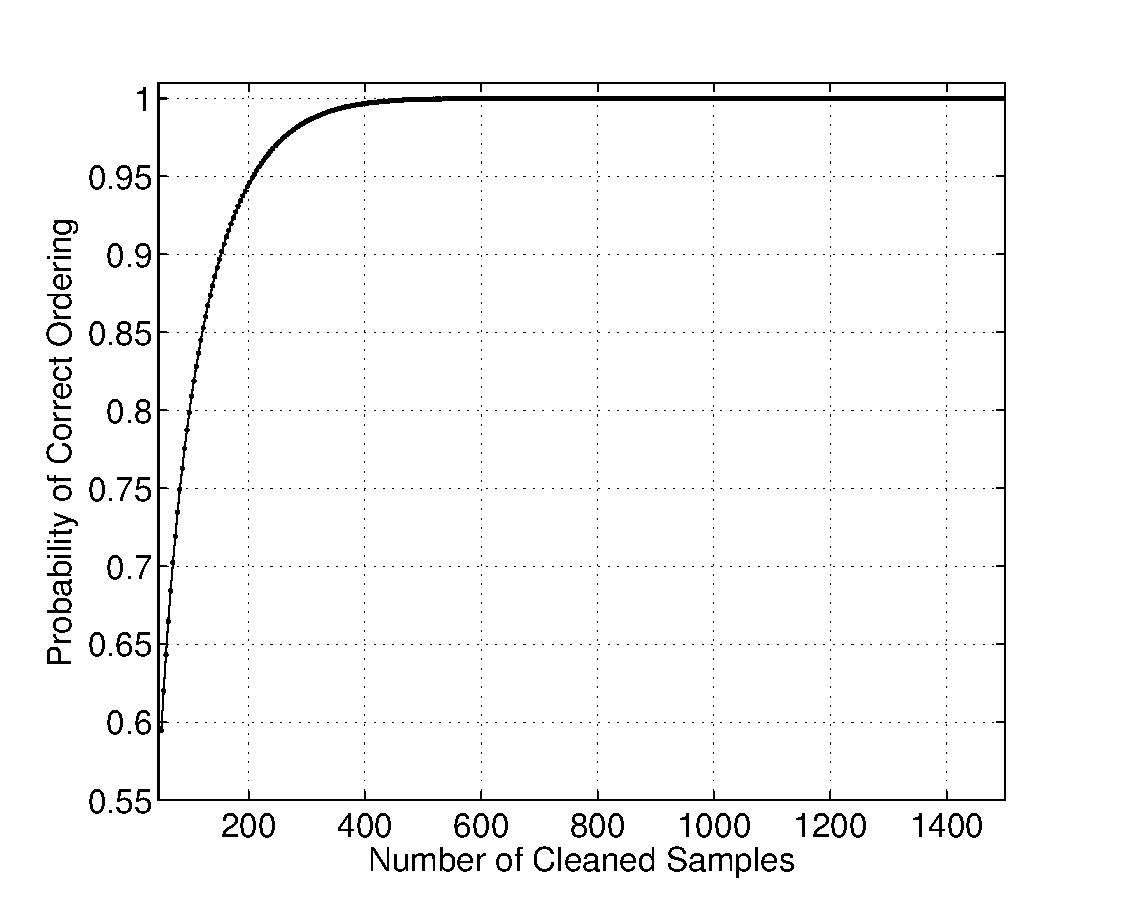
\includegraphics[width=0.3\textwidth]{figs/msacademic-paper-ranking.eps}

\begin{minipage}[b]{0.60\textwidth}
\centering
\scriptsize
\begin{tabular}{r r r r r}
\hline\hline
Name & Dirty & Clean & Pred \% & Dup \\ 
\hline  % inserts single horizontal line
Rakesh Agarwal & 353 & 211 & 18.13\% & 1.28\\
\hline
Jeffery Ullman & 460 & 255 & 05.00\% & 1.65\\
\hline
Michael Franklin & 560 & 173 & 65.09\% & 1.13\\
\hline
%\hline %inserts single line
\end{tabular}
\par\vspace{0pt}
\end{minipage}

%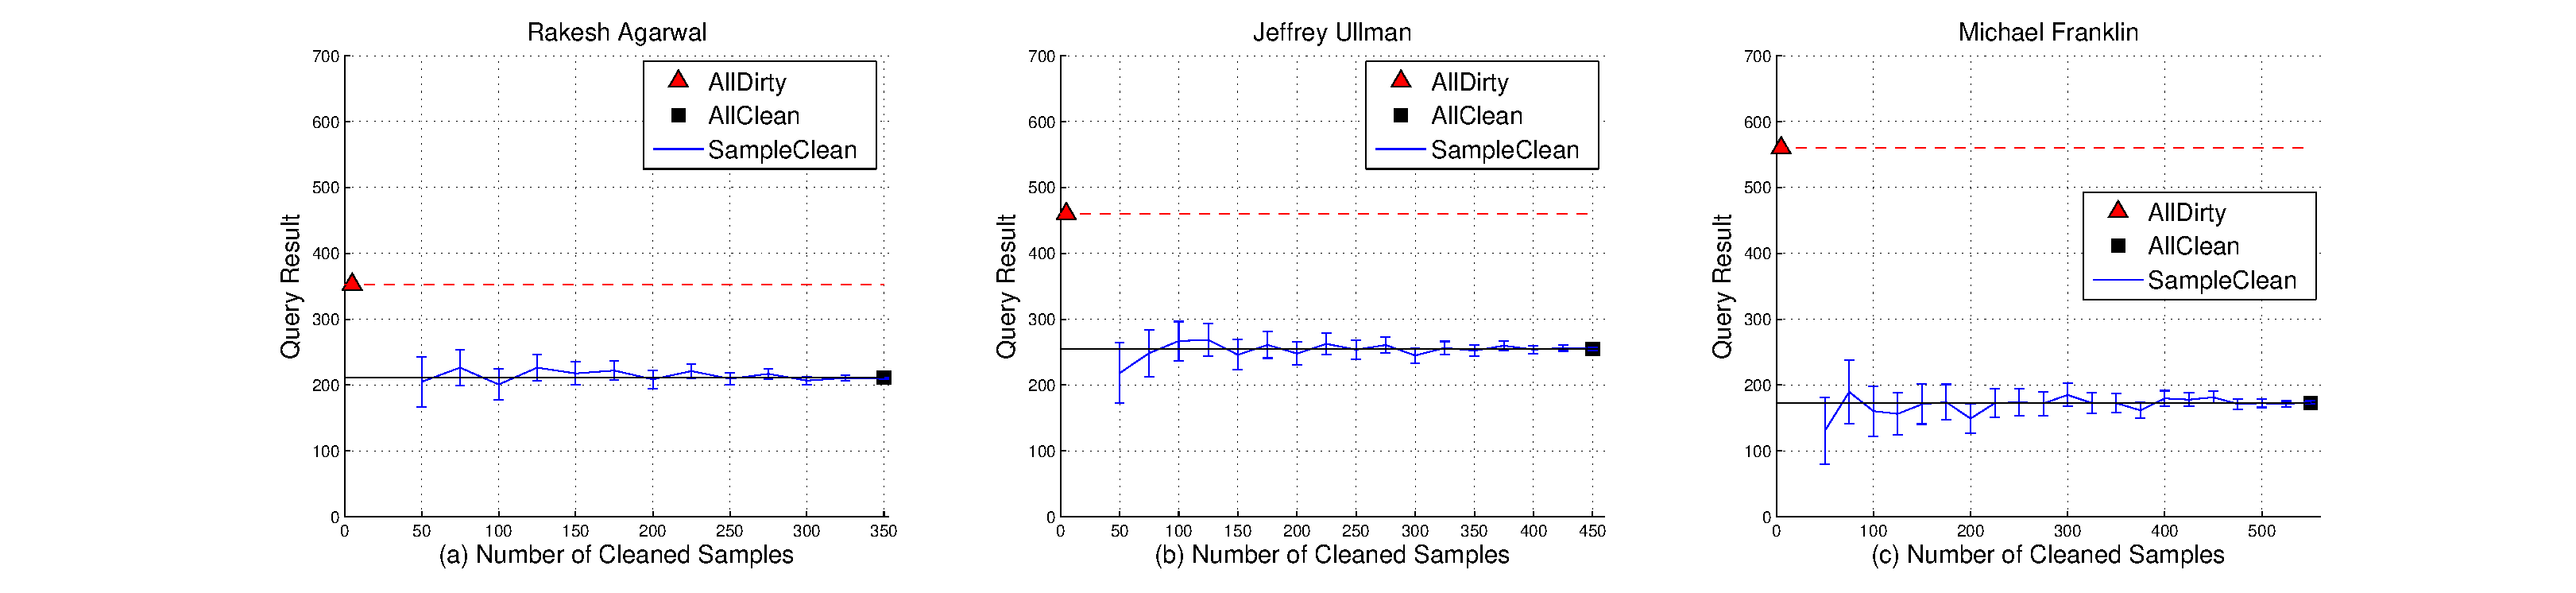
\includegraphics[width=0.78\textwidth]{figs/msacademic-paper-count.eps}

\caption{We can return the correct ranking with 95\% probability after cleaning only 210 total samples. To achieve a correct ranking with 99\% probability, we require 326 samples to be cleaned.\label{exp:ms-academic-ranking}}

\end{figure}



\section{View Cleaning: Scale View as Dirty Data \cite{krishnan2015svc}}
In follow-up work, we explored the generalization of \sampleclean.
Suppose the relation $R$ is in fact a derived relation $V$ of an underlying dirty database $D$.
We explored how we can efficiently apply a data cleaning operation to a sample of $V$.
This extension has an important application in approximate Materialized View maintenance, where we model a stale Materialized View as dirty data, and the maintenance procedure as cleaning.  

\subsection{Motivation}
There has been significant research on fast MV maintenance algorithms, most recently DBToaster \cite{DBLP:journals/vldb/KochAKNNLS14} which uses SQL query compilation and higher-order maintenance.
However, even with these optimizations, some materialized views are computationally difficult to maintain and will have maintenance costs that can grow with the size of data (e.g, correlated aggregate in a sub-query).
When faced with such challenges, it is common to batch updates to amortize maintenance overheads and add flexibility to scheduling.
Like dirty data, any amount of staleness can lead to erroneous query results where the user has no idea about the magnitude or the scope of query error. 
Thus, we explore how samples of ``clean" (up-to-date) data can be used for improved query processing on MVs without incurring the full cost of maintenance.

\subsection{Notation and Definitions}\label{notation}
\svc returns a bounded approximation for aggregate queries on stale MVs for a flexible additional maintenance cost.

\noindent \textbf{Materialized View:} Let $\mathcal{D}$ be a database which is a collection of relations $\{R_i\}$. 
A \emph{materialized view} $V$ is the result of applying a \emph{view definition} to $\mathcal{D}$. 
View definitions are composed of standard relational algebra expressions: Select ($\sigma_{\phi}$), Project ($\Pi$), Join ($\bowtie$), Aggregation ($\gamma$), Union ($\cup$), Intersection ($\cap$) and Difference ($-$). 

\vspace{0.5em}

\noindent \textbf{Primary Key:} We assume that each of the base relations has a \emph{primary key}. If this is not the case, we can always add an extra column that assigns an increasing sequence of integers to each record. 
This primary key is formally a subset of attributes $u \subseteq \{a_1,a_2,...,a_k\}$ such that all $s \in V(u)$ are unique.

\vspace{0.5em}

\noindent \textbf{Staleness:} For each relation $R_i$ there is a set of insertions $\Delta R_i$ (modeled as a relation)
and a set of deletions $\nabla R_i$.
An ``update'' to $R_i$ can be modeled as a deletion and then an insertion.
We refer to the set of insertion and deletion relations as ``delta relations", denoted by $\partial \mathcal{D}$:
\[
	\partial \mathcal{D} = \{\Delta R_1,...,\Delta R_k\} \cup \{\nabla R_1,...,\nabla R_k\}
\]
A view $S$ is considered \emph{stale} when there exist insertions or deletions to any of its base relations.
This means that at least one of the delta relations in $\partial \mathcal{D}$ is non-empty.

\vspace{0.5em}

\noindent \textbf{Maintenance:} There may be multiple ways (e.g., incremental maintenance or re-computation) to maintain a view $V$, and we denote the up-to-date view as $V'$.
We formalize the procedure to maintain the view as a \emph{maintenance strategy} $\mathcal{M}$.
A maintenance strategy is a relational expression the execution of which will return $V'$.
It is a function of the database $\mathcal{D}$, the stale view $V$, and all the insertion and deletion relations $\partial \mathcal{D}$. 
In this work, we consider maintenance strategies composed of the same relational expressions as materialized views described above.
\[
V' = \mathcal{M}(V,\mathcal{D}, \partial D)
\]

\vspace{0.5em}

\noindent \textbf{Staleness as Data Error:} The consequences of staleness are incorrect, missing, and superfluous rows. 
Formally, for a stale view $V$ with primary key $u$ and an up-to-date view $V'$:
\begin{itemize}[noitemsep] \sloppy
	\item \textbf{Incorrect: } Incorrect rows are the set of rows (identified by the primary key) that are updated in $V'$. For $v \in V$, let $v(u)$ be the value of the primary key. An incorrect row is one such that there exists a $v' \in V'$ with $v'(u) = V(u)$ and $v \ne v'$.
	\item \textbf{Missing: } Missing rows are the set of rows (identified by the primary key) that exist in the up-to-date view but not in the stale view. For $v' \in V'$, let $v'(u)$ be the value of the primary key. A missing row is one such that there does not exist a $v \in V$ with $v(u) = v'(u)$.
	\item \textbf{Superfluous: } Superfluous rows are the set of rows (identified by the primary key) that exist in the stale view but not in the up-to-date view. For $v \in V$, let $v(u)$ be the value of the primary key. A superfluous row is one such that there does not exist a $v' \in V'$ with $v(u) = v'(u)$.
\end{itemize}

\vspace{0.5em}

\noindent \textbf{Uniform Random Sampling:}
We define a sampling ratio $m\in [0,1]$ and for each row in a view $V$, we include it into a sample with probability $m$.
The relation $S$ is a \emph{uniform sample} of $V$ if
\[\text{(1) } \forall s \in S : s \in V\text{;~~~~~ (2) }Pr(s_1 \in S) =  Pr(s_2 \in S) = m.\]

\vspace{0.5em}

We say a sample is \emph{clean} if and only if it is a uniform random sample of the up-to-date view $V'$. 

\subsection{Problem Setup}
Formally, the workflow of \svc is:\vspace{-0.5em}
\begin{enumerate}[noitemsep]
\item We are given a view $V$.
\item $\mathcal{M}$ defines the maintenance strategy that updates $V$ at each maintenance period.
\item The view $V$ is stale between periodic maintenance, and the up-to-date view should be $V'$.
\item \emph{Stale Sample View Cleaning} We find an expression $\mathcal{C}$ derived from $\mathcal{M}$ 
that cleans a uniform random sample of the stale view $V$ to produce a ``clean" sample of the up-to-date
view $S_{clean}$.
\item \emph{Query Result Estimation} Given an aggregate query $q$ and the state query result $q(S)$, we use $S_{clean}$ and $S$ to estimate the up-to-date result. 
\end{enumerate} 

\vspace{0.25em}
\noindent\textbf{Stale View Cleaning Problem: }\sloppy
We are given a stale view $S$, a sample of this stale view $S$ with ratio $m$, the maintenance strategy $\mathcal{M}$, the base relations $\mathcal{D}$, and
the insertion and deletion relations $\partial \mathcal{D}$.
We want to find a relational expression $\mathcal{C}$ such that:
\[
V' = \mathcal{C}(S,\mathcal{D},\partial \mathcal{D}),
\]
where $V'$ is a sample of the up-to-date view with ratio $m$. 

\noindent\textbf{Query Result Estimation: }
The second problem addressed in this paper is query result estimation.
This problem can be addressed with the direct estimation and correction techniques 
described previously.

\subsection{Cleaning a Sample View}
To setup the problem, we first consider two naive solutions to this problem that will not work. 
We could trivially apply $\mathcal{M}$ to the entire stale view $S$ and update it to $V'$, and then sample.
While the result is correct according to our problem formulation, it does not save us on any computation for maintenance.
We want to avoid materialization of up-to-date rows outside of the sample. 
However, the naive alternative solution is also flawed. 
For example, we could just apply $\mathcal{M}$ to the stale sample $S$ and a sample of the delta relations $\widehat{\partial \mathcal{D}}$. 
The challenge is that $\mathcal{M}$ does not always commute with sampling.

\vspace{0.5em} 

\noindent\textbf{Provenance: } To address the commutativity problem, we need to ensure that for each $s \in V'$ all contributing rows in subexpressions to $s$ are also sampled. 
Provenance, also termed lineage, has been an important tool in the analysis of materialized views \cite{DBLP:journals/vldb/CuiW03} and in approximate query processing \cite{DBLP:conf/sigmod/ZengGMZ14}. 
We recursively define a set of primary keys for all relations in the expression tree to define tuple provenance:
\begin{definition} [Primary Key Generation]\label{pk}
For every relational expression $R$, we define the primary key attribute(s) of every expression to be:
\begin{itemize}[noitemsep]
\item Base Case: All relations (leaves) must have an attribute $p$ which is designated as a primary key. 
\item $\sigma_{\phi}(R)$: Primary key of the result is the primary key of R 
\item $\Pi_{(a_1,...,a_k)}(R)$: Primary key of the result is the primary key of R. The primary key must always be included in the projection.
\item $\bowtie_{\phi (r1,r2)}(R_1,R_2)$: Primary key of the result is the tuple of the primary keys of $R_1$ and $R_2$. 
\item $\gamma_{f,A}(R)$: The primary key of the result is the group by key $A$ (which may be a set of attributes).
\item $R_1 \cup R_2$: Primary key of the result is the union of the primary keys of $R_1$ and $R_2$
\item $R_1 \cap R_2$: Primary key of the result is the intersection of the primary keys of $R_1$ and $R_2$
\item $R_1 - R_2$: Primary key of the result is the primary key of $R_1$
\end{itemize}
For every node at the expression tree, these keys are guaranteed to uniquely identify a row.
\end{definition}
These rules define a constructive definition that can always be applied for our defined relational expressions. 

\vspace{0.5em} 

\noindent\textbf{Hashing: } The primary keys allow us to determine the set of rows that contribute to a row $r$ in a derived relation.
If we have a deterministic way of mapping a primary key to a Boolean, we can ensure that all contributing rows are also sampled. 
To achieve this we use a hashing procedure.
Let us denote the hashing operator $\eta_{a, m}(R)$. 
For all tuples in R, this operator applies a hash function whose range is $[0,1]$ to primary key $a$ (which may be a set) and selects those records with hash less than or equal to $m$.
To avoid materializing extra rows, we push down the hashing operator through the expression tree:
\begin{definition}[Hash push-down]
For a derived relation $R$, the following rules can be applied to push $\eta_{a, m}(R)$ down the expression tree. 
\begin{itemize}[noitemsep]
\item $\sigma_{\phi}(R)$: Push $\eta$ through the expression.  
\item $\Pi_{(a_1,...,a_k)}(R)$: Push $\eta $ through if $a$ is in the projection.
\item $\bowtie_{\phi (r1,r2)}(R_1,R_2)$: No push down in general. There are special cases below where push down is possible.
\item $\gamma_{f,A}(R)$: Push $\eta $ through if $a$ is in the group by clause $A$.
\item $R_1 \cup R_2$: Push $\eta $ through to both $R_1$ and $R_2$
\item $R_1 \cap R_2$: Push $\eta $ through to both $R_1$ and $R_2$
\item $R_1 - R_2$: Push $\eta $ through to both $R_1$ and $R_2$
\end{itemize}
\end{definition}

\noindent \textbf{Special Case of Joins: }
In general, a join $R \bowtie S$ blocks the push-down of the hash operator $\eta_{a, m}(R)$ since $a$ possibly consists of attributes in both $R$ and $S$.
However, when there is a constraint that enforces these attributes are equal then push-down is possible.

\emph{Foreign Key Join. } If we have a join with two foreign-key relations $R_1$ (fact table with foreign key $a$) and $R_2$ (dimension table with primary key $b \subseteq a$) and we are sampling the key $a$, then we can push the sampling down to $R_1$. This is because we are guaranteed that for every $r_1\in R_1$ there is only one $r_2 \in R_2$. 

\emph{Equality Join. } If the join is an equality join and $a$ is one of the attributes in the equality join condition $R_1.a = R_2.b$, then $\eta$ can be pushed down to both $R_1$ and $R_2$. On $R_1$ the pushed down operator is $\eta_{a, m}(R_1)$ and on $R_2$ the operator is $\eta_{b, m}(R_2)$.

\vspace{0.5em} 

\noindent \textbf{Efficient View Cleaning: }
If we apply the hashing operator to $\mathcal{M}$, we can get an optimized cleaning expression $\mathcal{C}$ that avoids materializing unnecessary rows. 
When applied to a stale sample of a view $S$, the database $\mathcal{D}$, and the delta relations $\partial \mathcal{D}$, it produces an up-to-date sample with sampling ratio $m$:
\[
V' = \mathcal{C}(S,\mathcal{D},\partial \mathcal{D})
\]
Thus, it addresses Problem 1, and with the materialized sample of up-to-date rows, we can apply the direct estimates and corrections in the previous section to estimate the result bounded in confidence intervals.

\subsection{Results: Video Streaming Log Analysis}
We evaluate \svc on Apache Spark~1.1.0 with 1TB of logs from a video streaming company, Conviva \cite{conviva}.
This is a denormalized user activity log corresponding to video views and various metrics such as data transfer rates, and latencies.
Accompanying this data is a four month trace of queries in SQL.
We identified 8 common summary statistics-type queries that calculated engagement and error-diagnosis metrics.
We populated these view definitions using the first 800GB of user activity log records.  
We then applied the remaining 200GB of user activity log records as the updates (i.e., in the order they arrived) in our experiments.
We generated aggregate random queries over this view by taking either random time ranges or random subsets of customers.

\begin{figure}[t]
\centering
 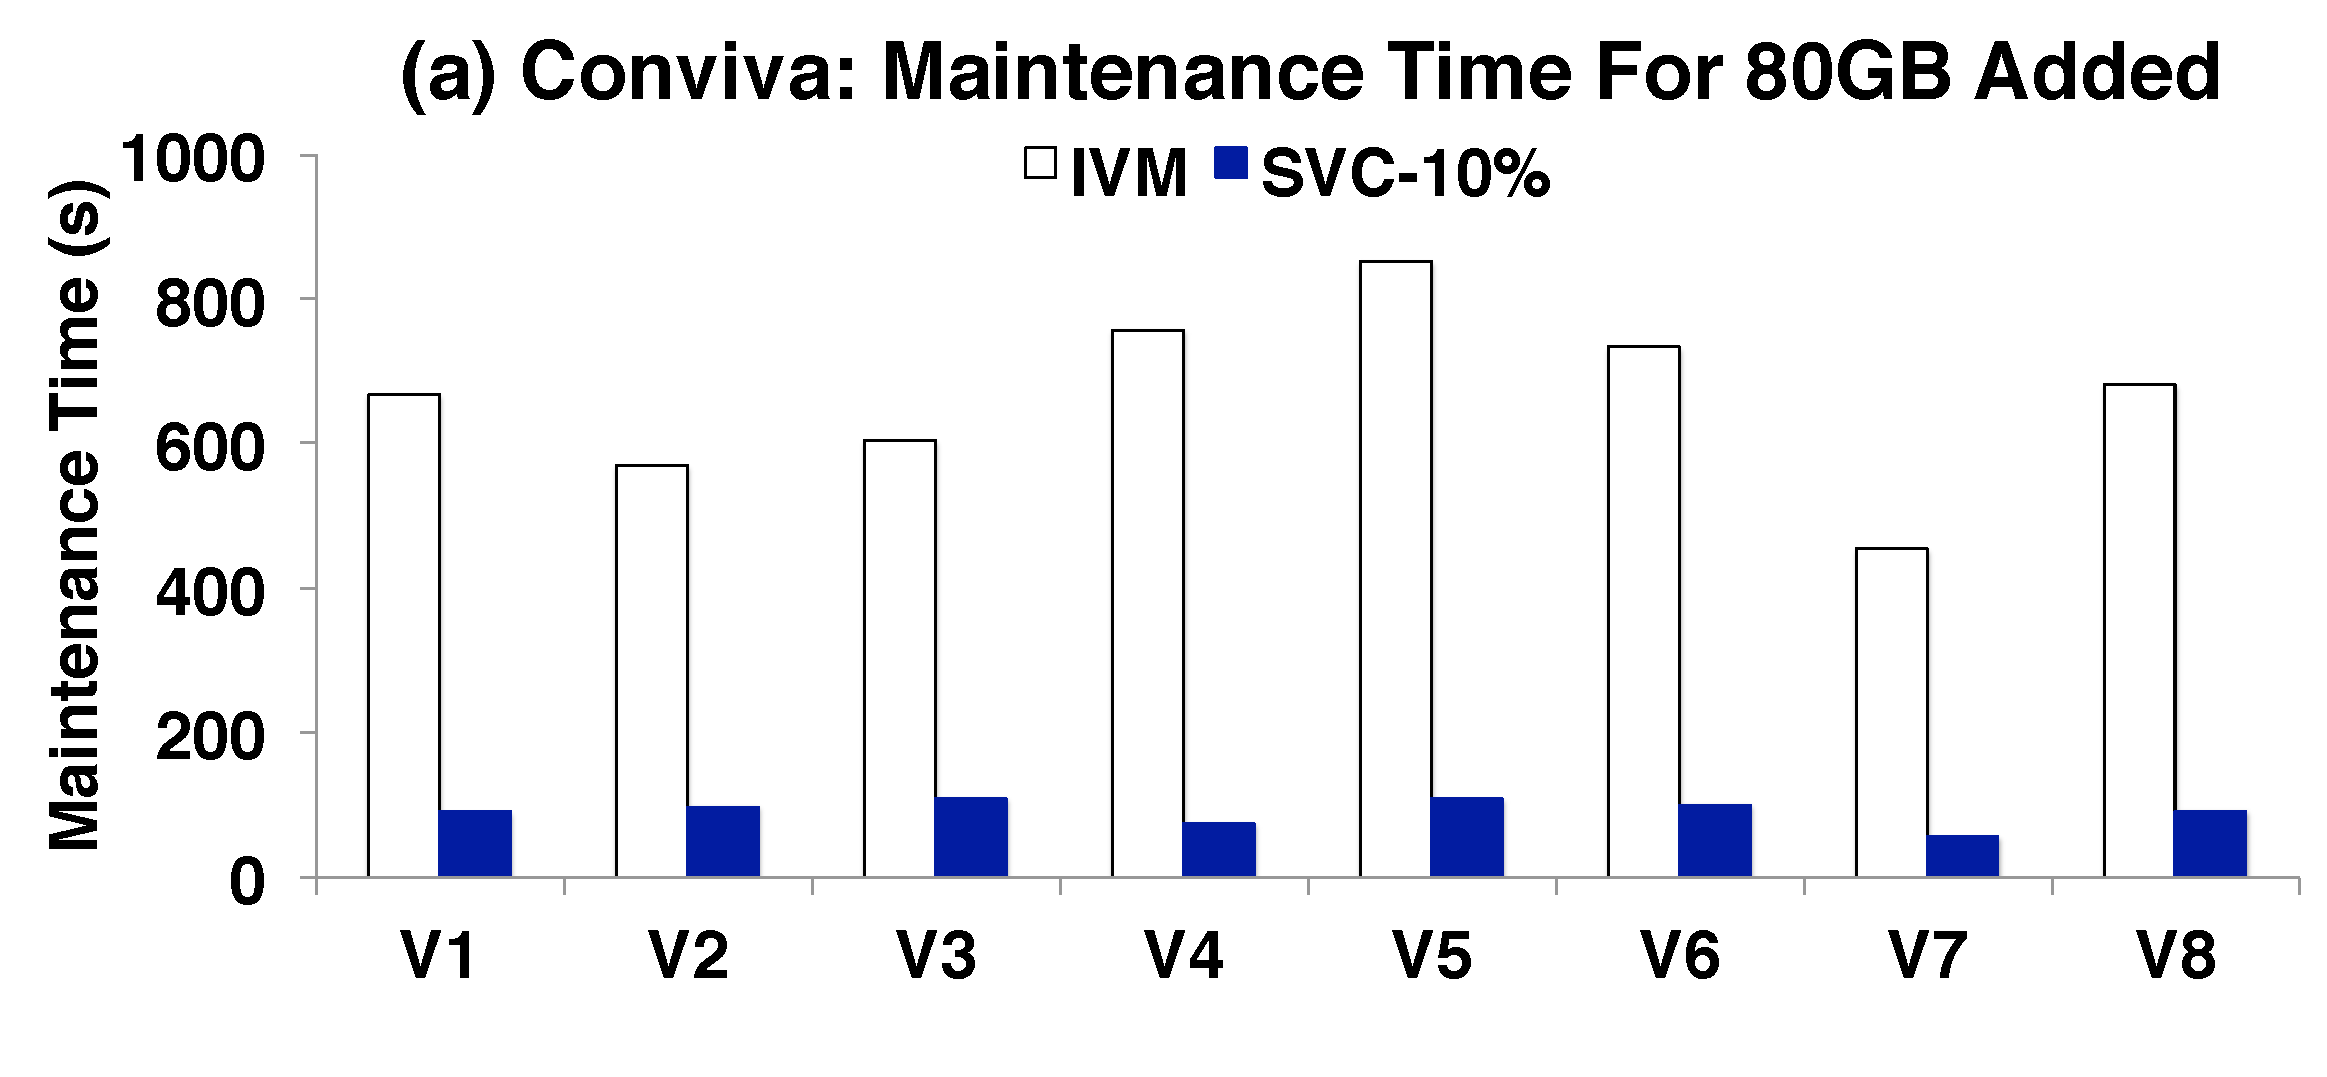
\includegraphics[scale=0.16]{figs/con_3.pdf}
 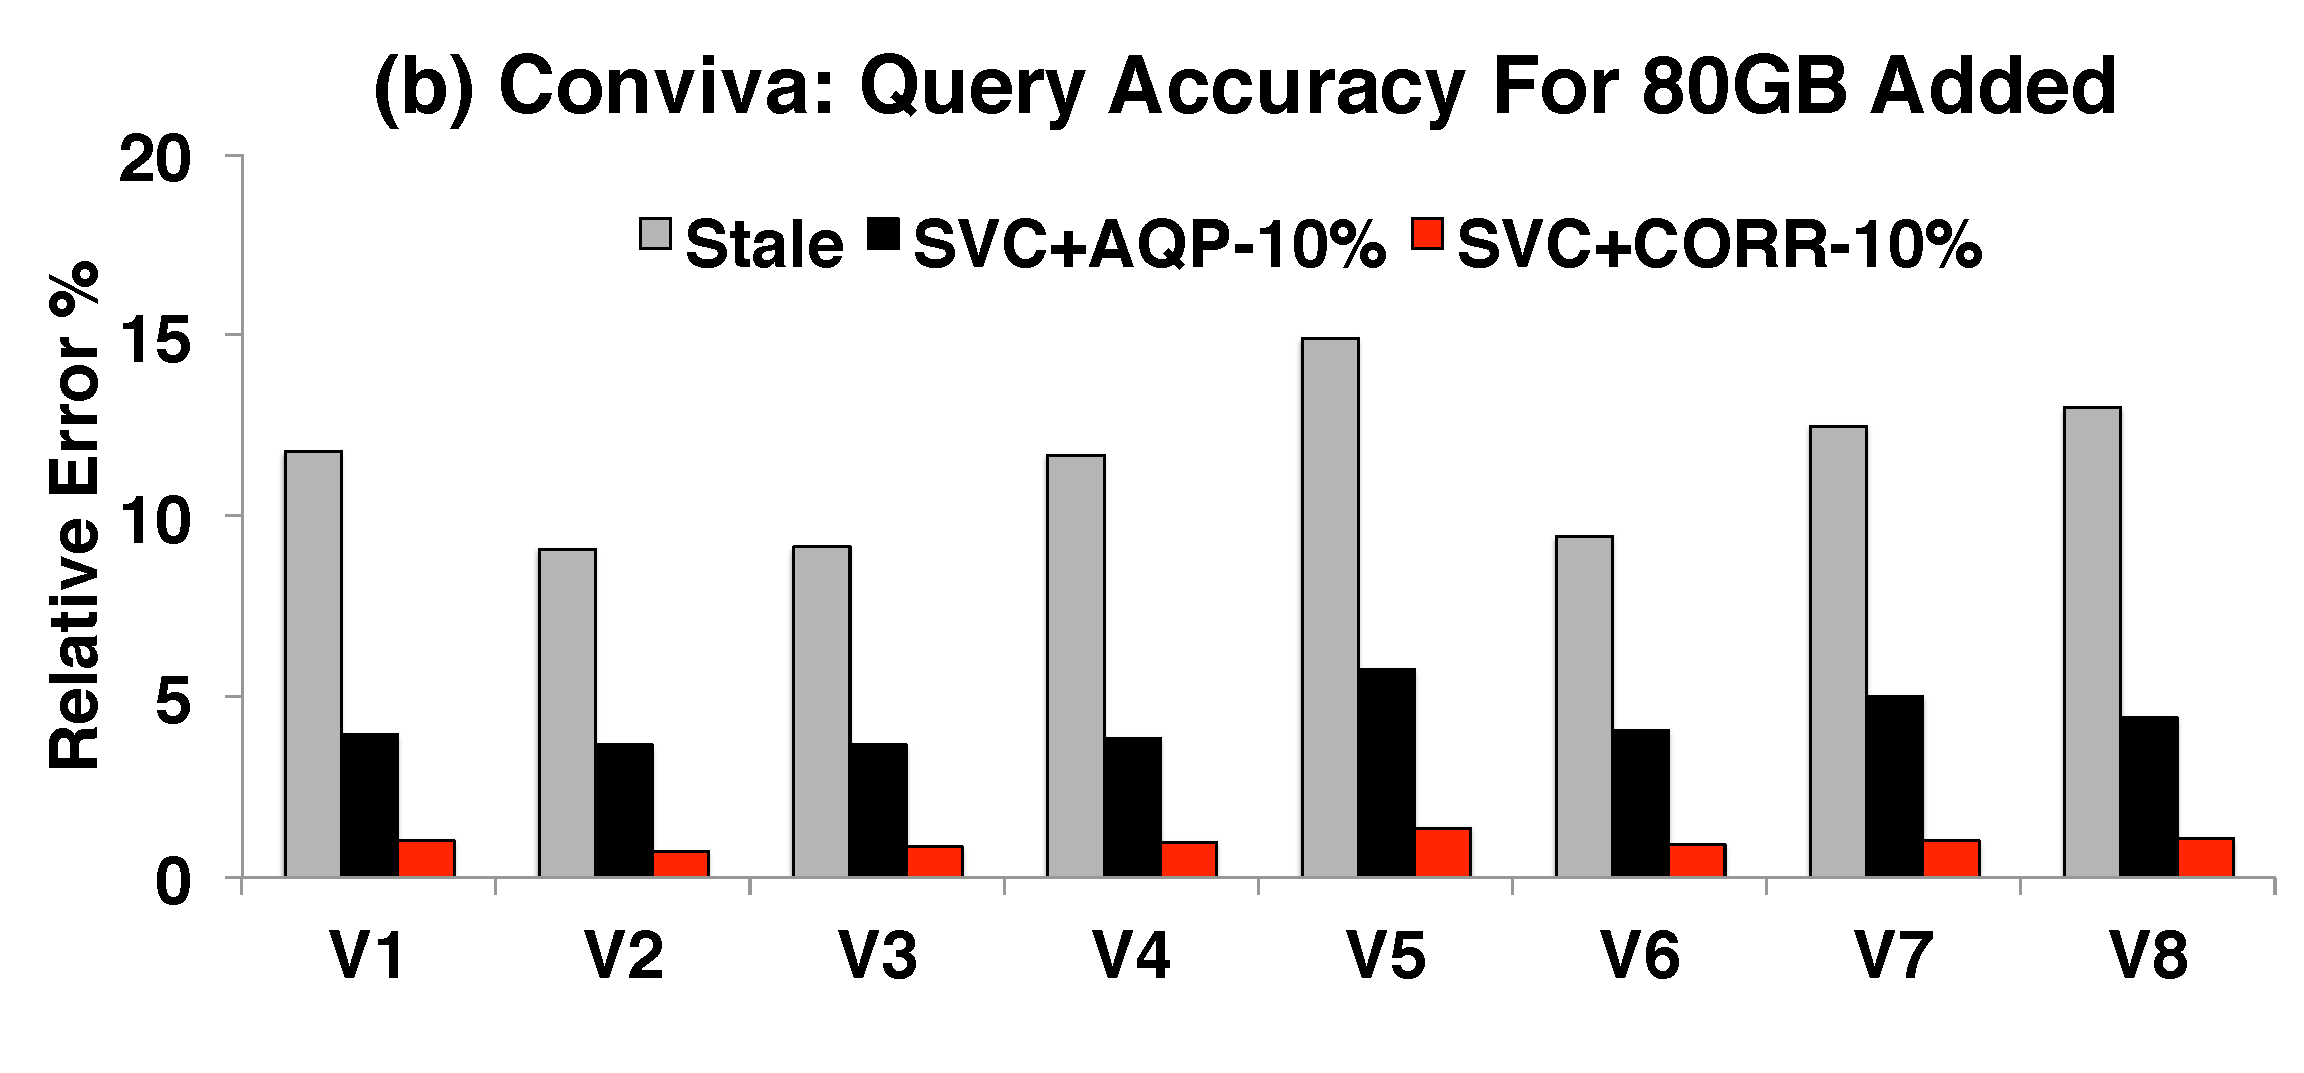
\includegraphics[scale=0.16]{figs/con_4.pdf} \vspace{-1.5em}
 \caption{(a) We compare the maintenance time of \svc with a 10\% sample and full incremental maintenance (IVM). (b) We also evaluate the accuracy of the estimation techniques: (Direct DIR), Correction (CORR), and Dirty (Stale). \label{conv-1}}\vspace{-1.5em}
\end{figure}

In Figure \ref{conv-1}(a), we show that on average over all the views, \svc with a 10\% sample gives a 7.5x speedup.
For one of the views full incremental maintenance takes nearly 800 seconds, even on a 10-node cluster, which is a very significant cost.
In Figure \ref{conv-1}(b), we show that \svc also gives highly accurate results with an average error of 0.98\% for the correction estimate.
This experiment highlights a few salient benefits of \svc: (1) sampling is a relatively cheap operation and the relative speedups in a single node and distributed environment are similar, (2) for analytic workloads like Conviva (i.e., user engagement analysis) a 10\% sample gives results with 99\% accuracy, and (3) savings are still significant in systems like Spark that do not support selective updates.


\section{ActiveClean: Machine Learning on Dirty Data}
Analytics is moving beyond SQL, and the growing popularity of predictive models \cite{bdas, alexandrov2014stratosphere, crotty2014tupleware, hellerstein2012madlib} leads to additional challenges in managing dirty data.

\subsection{Simpson's Paradox}
The challenge is that the high-dimensional models are very sensitive to systematic biases, and many of the techniques applied in practice suffer methodological problems.
One technique to avoid dependence on sample size is ``write back" approach, where $k$ rows are cleaned and written back to the database.
Let $k$ rows be cleaned, but all of the remaining dirty rows are retained in the dataset.
Figure \ref{update-arch1} highlights the dangers of this approach on a very simple dirty dataset and a linear regression model i.e., the best fit line for two variables. 
One of the variables is systematically corrupted with a translation in the x-axis (Figure \ref{update-arch1}a).
The dirty data is marked in brown and the clean data in green, and their respective best fit lines are in blue.
After cleaning only two of the data points (Figure \ref{update-arch1}b), the resulting best fit line is in the opposite direction of the true model.
This is a well-known phenomenon called Simpsons paradox, where mixtures of different populations of data can result in spurious relationships \cite{simpson1951interpretation}.
Training models on a mixture of dirty and clean data can lead to unreliable results, where artificial trends introduced by the mixture can be confused for the effects of data cleaning.
Figure \ref{update-arch1}c also illustrates that, even in two dimensions, models trained from small samples can be as incorrect as the mixing solution described before.

\begin{figure}[ht!]
\centering
 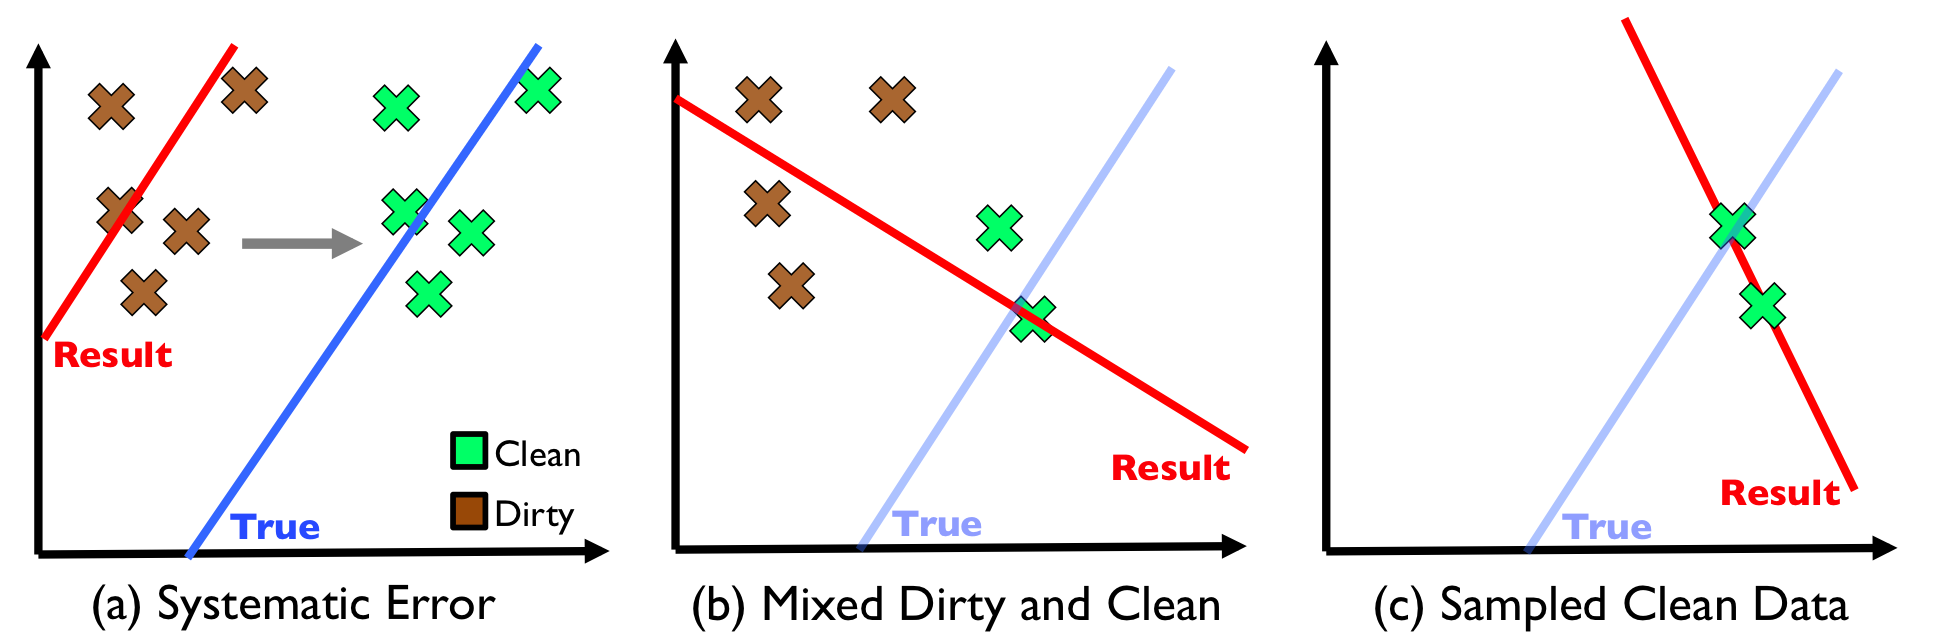
\includegraphics[width=0.6\columnwidth]{figs/update-arch.png}
 \caption{(a) Systematic corruption in one variable can lead to a shifted model. 
 (b) Mixed dirty and clean data results in a less accurate model than no cleaning.
(c) Small samples of only clean data can result in similarly inaccurate models. \label{update-arch1}}
\end{figure}

\subsection{Problem Setup}
This work focuses on a class of well analyzed predictive analytics problems; ones that can be expressed as the minimization of convex loss functions.
Examples includes all generalized linear models (including linear and logistic regression), all variants of support vector machines, and in fact, \avgfunc and \medfunc are also special cases. 

Formally, for labeled training examples $\{(x_{i},y_{i})\}_{i=1}^{N}$, the problem is to find a vector of \emph{model parameters} $\theta$ by minimizing a loss function $\phi$ over all training examples:
\[
 \theta^{*}=\arg\min_{\theta}\sum_{i=1}^{N}\phi(x_{i},y_{i},\theta)
\]
Where $\phi$ is a convex function in $\theta$.
Without loss of generality, we will include regularization as part of the loss function i.e., $\phi(x_{i},y_{i},\theta)$ includes $r(\theta)$.

\begin{definition}[Convex Data Analytics]
A convex data analytics problem is specified by a set of features $X$, corresponding set of labels $Y$, and a parametrized loss function $\phi$ that is convex in its parameter $\theta$.
The result is a \textbf{model} $\theta$ that minimizes the sum of losses over all features and labels.
\end{definition}

\vspace{0.5em}
\noindent\textbf{ActiveClean Problem: }\label{activeclean}\sloppy
Let $R$ be a dirty relation, $F(r) \mapsto (x,y)$ be a featurization that maps
a record $r \in R$ to a feature vector $x$ and label $y$, $\phi$ be a convex regularized loss,
and $C(r) \mapsto r_{clean}$ be a cleaning technique that maps a record to its cleaned value. 
Given these inputs, the ActiveClean problem is to return a \textbf{reliable} estimate $\hat{\theta}$ of the clean model for any limit $k$ on the number of times the data cleaning $C(\cdot)$ can be applied.

\vspace{0.25em}

\emph{Reliable} precisely means that the expected error in this estimate (i.e., L2 difference w.r.t a model trained on a fully cleaned dataset) is bounded above by a monotonically decreasing function in $k$ and a monotonically decreasing function of the error of the dirty model. In other words, more cleaning implies more accuracy, and less initial error implies faster convergence.

\subsection{Model Updates}
The main insight of this work is that, in Convex Data Analytics, sampling is naturally part of the query processing.
Mini-batch stochastic gradient descent (SGD) is an algorithm for finding the optimal value
given the convex loss and data.
In mini-batch SGD, random subsets of data are selected at each iteration and the average gradient is computed for every batch.
Instead of calculating the average gradient for the batch w.r.t to the dirty data, we apply data cleaning at that point--inheriting the convergence bounds from batch SGD.
It is well known that even for an arbitrary initialization SGD makes significant progress in less than one epoch (a pass through the entire dataset) \cite{bottou2012stochastic}.
Furthermore in this setting, the dirty model can be much more accurate than an arbitrary initialization; leading to highly accurate models without processing the entire data.

ActiveClean is initialized with $\theta^{(1)} = \theta^{(d)}$ which is the dirty model.
At each iteration $t=\{1,...,T\}$, the cleaning is applied to a batch of data $b$ selected from the set of candidate dirty rows $R$.
Then, an average gradient is estimated from the cleaned batch and the model is updated.
Iterations continue until $k = T \cdot b$ rows are cleaned.

\begin{enumerate}[noitemsep]
	\item Calculate the gradient over the sample of clean data and call the result $g_S(\theta^{(t)})$
	\item Apply the following update rule:
	\[
	\theta^{(t+1)} \leftarrow \theta^{(t)} - \lambda \cdot g_S(\theta^{(t)}) 
	\]
\end{enumerate} 

\subsection{Optimizations}
ActiveClean has a number of additional optimizations exploiting the structure of Convex Data Analytics problems.

\noindent\textbf{Detector: } In this step, the detector select a candidate set of dirty rows $R_{dirty} \subseteq R$. There are two techniques to do this: (1) an \emph{a priori} case, and (2) and an adaptive case. In the \emph{a priori} case, the detector knows which data is dirty in advance. In the adaptive case, the detector learns classifier based on previously cleaned data to detect corruption in uncleaned data. This allows ActiveClean to prioritize cleaning data expected to be dirty. 

\vspace{0.5em}

\noindent\textbf{Non-uniform Sampler: } The sampler draws a sample of rows $S_{dirty} \subseteq R_{dirty}$. This is a non-uniform sample where each record $r$ has a sampling probability $p(r)$.
We derive the theoretical minimum variance sampling distribution, which is impossible to realize as it requires knowing the clean data in advance. Therefore, we use a first order first-order approximation of this distribution based on estimates of the clean data. 

\vspace{0.5em}

\noindent\textbf{Estimator: } The estimator approximates the optimal distribution derived in the Sample step. Based on the change in the featurized data $F(S_{clean})$ and $F(S_{dirty})$, it directs the next iteration of sampling to select points that will have changes most valuable to the next model update.




\section{Related Work}
{\noindent \bf Approximate Query Processing:} AQP has been studied for more than two decades~\cite{DBLP:conf/vldb/GarofalakisG01,DBLP:journals/ftdb/CormodeGHJ12}.
Many AQP approaches~\cite{DBLP:journals/tods/ChaudhuriDN07,DBLP:conf/eurosys/AgarwalMPMMS13,DBLP:conf/sigmod/AcharyaGPR99,DBLP:conf/cidr/SidirourgosKB11,DBLP:conf/sigmod/BabcockCD03,DBLP:conf/sigmod/HellersteinHW97,DBLP:journals/pvldb/PansareBJC11,DBLP:conf/sigmod/CondieCAHGTES10,DBLP:journals/pvldb/WuJOT09} were proposed, aiming to enable interactive query response times.
%Acharya et al.~\cite{DBLP:conf/sigmod/AcharyaGPR99} developed the Aqua system which is run on top of relational DBMS, and allows users to obtain approximate query answers in a fast response time. Chaudhuri et al.~\cite{DBLP:journals/tods/ChaudhuriDN07} studied how to create an optimal stratified random sample based on a given query workload, and proposed the STRAT algorithm that can make the workload queries achieve the best quality on the sample. Sidirourgos et al.~\cite{DBLP:conf/cidr/SidirourgosKB11} presented the SciBORQ architecture that creates biased multi-layered samples based on the scientific data exploration workload, and adaptively select a suitable sample to satisfy quality or time constraints during query execution. Agarwal et al.~\cite{DBLP:conf/eurosys/AgarwalMPMMS13} devised novel multi-dimensional stratified samples based on real-world big data analytics workloads, and built the BlinkDB system to utilize the created samples to support interactive query processing with error and response time constraints. Unlike the above approaches which create samples ahead of query time, online aggregation~\cite{DBLP:conf/sigmod/HellersteinHW97,DBLP:journals/pvldb/PansareBJC11,DBLP:conf/sigmod/CondieCAHGTES10,DBLP:journals/pvldb/WuJOT09} constructs samples in an online fashion, and gradually achieve more and more accurate results until users are satisfied about the current results. 
There are also many studies on creating other synopsis of the data, such as histograms or wavelets~\cite{DBLP:journals/ftdb/CormodeGHJ12}. While a substantial works on approximate query processing, these works mainly focus on how to deal with sampling errors, with little attention to data errors. 

\vspace{.5em}

{\noindent \bf Data Cleaning:} There have been many studies on various data-cleaning techniques, such as rule-based approaches~\cite{fan2012foundations,DBLP:conf/sigmod/DallachiesaEEEIOT13}, outlier detection~\cite{hellerstein2008quantitative,dasu2003exploratory}, filling missing values, and duplicate detection~\cite{conf/hdkm/Christen08, DBLP:conf/kdd/BilenkoM03, conf/sigmod/WangLF12}. In order to ensure reliable cleaning results, most of these techniques require human involvement~\cite{DBLP:conf/sigmod/JefferyFH08,DBLP:journals/pvldb/FanLMTY10,DBLP:journals/pvldb/YakoutENOI11,DBLP:journals/pvldb/WangKFF12,DBLP:conf/sigmod/WangLKFF13}. 
For example, Fan et al.~\cite{DBLP:journals/pvldb/FanLMTY10} proposed to employ editing rules, master data and user confirmation to clean data, and proved that their approaches can always lead to correct cleaning results. Wang et al.~\cite{DBLP:journals/pvldb/WangKFF12} proposed a hybrid human-machine approach to detect duplicate entities in data, which can achieve higher detection accuracy than machine-only approaches. 
In SampleClean, the main focus is not on a specific data-cleaning technique, but rather on a new framework that enables a flexible trade-off between data cleaning cost and result quality.
Indeed, we can apply any data-cleaning technique to clean the sample data, and then utilize our framework to estimate query results based on the cleaned sample. 

\vspace{.5em}

{\noindent \bf Views and Cleaning:} Meliou et al. \cite{DBLP:conf/sigmod/MeliouGNS11} proposed a technique to trace errors in an MV to base data and find responsible erroneous tuples. 
They do not, however, propose a technique to correct the errors as in \svc.
Correcting general errors as in Meliou et al. is a hard constraint satisfaction problem.
However, in \svc, through our formalization of staleness, we have a model of how updates to the base data (modeled as errors) affect MVs, which allows us to both trace errors and clean them.
Wu and Madden \cite{DBLP:journals/pvldb/0002M13} did propose a model to correct ``outliers" in an MV through deletion of records in the base data.
This is a more restricted model of data cleaning than \svc, where the authors only consider changes to existing rows in an MV (no insertion or deletion) and do not handle the same generality of relational expressions (e.g., nested aggregates).
Challamalla et al. \cite{DBLP:conf/sigmod/ChalamallaIOP14} proposed an approximate technique for specifying errors as constraints on a materialized view and proposing changes to the base data such that these constraints can be satisfied.
While complementary, one major difference between the three works \cite{DBLP:conf/sigmod/MeliouGNS11, DBLP:journals/pvldb/0002M13, DBLP:conf/sigmod/ChalamallaIOP14} and \svc is that they require an explicit specification of erroneous rows in a materialized view.
Identifying whether a row is erroneous requires materialization and thus specifying the errors is equivalent to full incremental maintenance. 
We use the formalism of a ``maintenance strategy", the relational expression that updates the view, to allow us to sample rows that are not yet materialized.
However, while not directly applicable for staleness, we see \svc as complementary to these works in the dirty data setting. 


\vspace{.5em}

{\noindent \bf Result Estimation and Sampling:}
Estimating aggregate statistics of populations from samples has been well studied in the field of surveying \cite{weisberg2009total,valliant2000finite, hansen1987some, barnett1991sample, sarndal2003model, kalton1983introduction}.
These works explore different types of sampling, error characterizations, bias-variance trade-offs, and confidence intervals.
The theoretical foundation of surveying is statistical bounding of functions of independent random variables (e.g., samples with replacement).
This field includes distribution-free bounds such as Markov/Chebyshev/Hoeffding bounds, asymptotic bounds such as the Central Limit Theorem (CLT), and empirical testing such as Bootstrapping \cite{hinkley1988bootstrap}.
For a detailed survey of different types of statistical bounds refer to \cite{hahn2011statistical}.
Due to the CLT's strong guarantees (unbiased sample estimates and normalcy), as in our work, it is widely applied in the analysis of sampling schemes.
The more general study of sample estimators that are unbiased and have asymptotically normal distributions (like the CLT) is called U-Statistics, refer to \cite{lee1990u} for a survey of this theory.
The stochastic process literature also discusses problems in unbiased estimation from samples \cite{jacod1987limit}.

\vspace{.5em}

{\noindent \bf Distinct Value Estimation:}
Distinct value estimation has been an open problem in stream processing and database research~\cite{considine2004approximate,bar2002counting,haas1995sampling,beyer2007synopses}.
Similar to our analysis, some have argued that simply removing duplicates in a sample of data does not work~\cite{charikar2000towards}.
In the storage literature, similar weighted average techniques have been applied for global file duplication rate estimation \cite{harnik2012estimation} based on the knowledge of duplication rates within a sample.
This work can be seen as a simplified version of our problem only answering a count query with only duplication errors.
Techniques similar to our duplicate reweighting scheme have been studied in estimating from non-uniform samples \cite{aldroubi2002non}, and is also similar to the acceptance ratio used sampling algorithms such as the Metropolis-Hastings Algorithm and Rejection Sampling \cite{liu1996metropolized,metropolis1953equation}.
Further relevant work includes sensitivity analysis of set functions \cite{mcdiarmid1989method, jukna2012analysis} and statistical information theory \cite{kullback1997information}. 

\section{Future Work and Open Problems}
We further describe a number of open theoretical and practical problems to challenge the community:

\vspace{0.5em}
\noindent \textbf{Completeness: } For aggregate queries in the budgeted data cleaning setting,
variance of the clean data $\sigma_c^2$, variance of the pairwise differences between clean and dirty data $\sigma_d^2$, and sample size $k$, is $O(\frac{\min \{\sigma_c,\sigma_d\}}{\sqrt{k}})$ (derived in this work) an optimal error bound?
It is clear than in the parametric setting, where it additional information known this is not true. For example, if we know that all of the data was on a single line then it would require only two clean attributes to reconstruct the entire distribution. 

\vspace{0.5em}
\noindent \textbf{Point-Lookup Dichotomy: } This work focuses on aggregate analytics such as queries and statistical models. In fact, as the selectivity of the analytics goes to 0 (i.e., single row lookup), the bounds in this work limit to infinity. However, in practice, cleaning a sample of data can be used to address such queries, where a statistical model can be trained on a sample of data to learn a mapping between dirty and clean data. An open problem is exploring how much looser is a generalization bound (e.g., via Learning Theory) compared to the bounds on aggregate queries.

\vspace{0.5em}
\noindent \textbf{Confirmation Bias and Sample Re-use: } In practice, users repeatedly query and clean the sample of data. As a result, estimates are highly correlated and potentially overfit to a sample. An open problem is designing efficient sampling techniques to mitigate the effects of \emph{confirmation bias} and discourage a user from overfitting analysis to the sample.

\vspace{0.5em}
\noindent \textbf{Sample-based Optimization of Workflows: } In practical data cleaning workflows, there are numerous design choices e.g., whether or not to use crowdsourcing, similarity functions, etc. An open problem is using samples of cleaned data to estimate and tune parameters on data cleaning workflows.

\vspace{0.5em}
\noindent \textbf{Black-box Applications: } SampleClean exploits the structure of the application to budget data cleaning. However, in some cases, the application is opaque with a UDF quality metric (i.e., number of complaints recieved from users). Is it possible to probe an application to understand which errors affect the application?

\vspace{0.5em}
\noindent \textbf{Simulation and Knowledge Bases: } A number of recent projects are curating large knowledge bases. These knowledge bases may be useful for simulation realistic data errors such as entity resolution and missing value problems. Is it possible to learn a data cleaning policy from simulation of examples?



\section{Conclusion}
An important challenge in data analytics is presence of dirty data
in the form of missing, duplicate, incorrect or inconsistent values.
Data analysts report that data cleaning remains one of the most time
consuming steps in the analysis process, and data cleaning can require
a significant amount of developer effort in writing software or rules
to fix the corruption. 
SampleClean studies the integration of Sample-based Approximate Query Processing and data cleaning; to provide analysts a tradeoff between cleaning the entire dataset and avoiding cleaning altogether.
To the best of our knowledge, this is the first work to marry data cleaning with sampling-based query processing.
While sampling introduces approximation error, the data cleaning mitigates errors in query results.
This idea opened up a number of new research opportunities, and we applied the same principles to other domains such as Materialized View Maintenance and Machine Learning.

\vspace{1.5em}

\textbf{\small This research is supported in part by NSF CISE Expeditions Award CCF-1139158, DOE Award SN10040 DE-SC0012463, and DARPA XData Award FA8750-12-2-0331, and gifts from Amazon Web Services, Google, IBM, SAP, The Thomas and Stacey Siebel Foundation, Adatao, Adobe, Apple, Inc., Blue Goji, Bosch, Cisco, Cray, Cloudera, EMC2, Ericsson, Facebook, Guavus, HP, Huawei, Informatica, Intel, Microsoft, NetApp, Pivotal, Samsung, Schlumberger, Splunk, Virdata and VMware.}


\fontsize{8.2pt}{8.4pt} \selectfont
\bibliographystyle{abbrv}
\bibliography{ref} 

\end{document}

